%%%%%%%%%%%%%%%%%%%%%%%%%%%%%%%%%%%%%%%%%%%%%%%%%%%%%%%%%%%%
% 1.2 LINEAR ALGEBRA
% The Composition of Advanced Mathematics
%%%%%%%%%%%%%%%%%%%%%%%%%%%%%%%%%%%%%%%%%%%%%%%%%%%%%%%%%%%%

\section{Linear Algebra}
\label{sec:linear-algebra}

\prerequisite{
Elementary algebra from \cref{sec:elementary-algebra}, functions from
\cref{sec:functions}, elementary set theory from
\cref{sec:elementary-set-theory}, and methods of proof from
\cref{sec:methods-of-proof}.
}

\learningobjectives{
By the end of this section, the reader should be able to:
\begin{itemize}
    \item interpret and solve systems of linear equations;
    \item visualize systems geometrically;
    \item represent systems using augmented matrices;
    \item perform elementary row operations;
    \item distinguish echelon form and reduced row-echelon form;
    \item identify pivot and free variables;
    \item write solution sets in parametric vector form;
    \item perform matrix arithmetic and matrix multiplication;
    \item interpret matrices as transformations;
    \item compute and interpret determinants;
    \item understand determinants as area and volume scaling;
    \item work with vectors geometrically and algebraically;
    \item interpret linear combinations, span, and linear independence;
    \item understand vector spaces and subspaces;
    \item identify bases and dimensions;
    \item understand row spaces, column spaces, and null spaces;
    \item interpret rank and nullity;
    \item understand linear transformations, kernels, and images;
    \item compute and interpret eigenvalues and eigenvectors;
    \item understand diagonalization;
    \item work with dot products, norms, angles, and orthogonality;
    \item compute vector projections;
    \item understand the geometric idea behind least-squares approximation.
\end{itemize}
}

%%%%%%%%%%%%%%%%%%%%%%%%%%%%%%%%%%%%%%%%%%%%%%%%%%%%%%%%%%%%
\subsection{What Is Linear Algebra?}
\label{subsec:what-is-linear-algebra}
%%%%%%%%%%%%%%%%%%%%%%%%%%%%%%%%%%%%%%%%%%%%%%%%%%%%%%%%%%%%

Linear algebra studies mathematical structures governed by two fundamental
operations:

\begin{itemize}
    \item addition;
    \item scalar multiplication.
\end{itemize}

Its central objects include

\begin{itemize}
    \item systems of linear equations;
    \item vectors;
    \item matrices;
    \item vector spaces;
    \item linear transformations;
    \item eigenvalues and eigenvectors.
\end{itemize}

\begin{conceptbox}
Linear algebra provides a language for describing multidimensional structure,
transformations, systems, and data.
\end{conceptbox}

%%%%%%%%%%%%%%%%%%%%%%%%%%%%%%%%%%%%%%%%%%%%%%%%%%%%%%%%%%%%
\subsection{Why Linear Algebra Matters}
\label{subsec:why-linear-algebra-matters}
%%%%%%%%%%%%%%%%%%%%%%%%%%%%%%%%%%%%%%%%%%%%%%%%%%%%%%%%%%%%

Linear algebra appears throughout mathematics and applied science.

Important applications include

\begin{itemize}
    \item differential equations;
    \item multivariable calculus;
    \item statistics and regression;
    \item numerical analysis;
    \item optimization;
    \item computer graphics;
    \item machine learning;
    \item network analysis;
    \item quantum mechanics;
    \item dynamical systems;
    \item data science.
\end{itemize}

Even nonlinear systems are often approximated locally by linear models.

%%%%%%%%%%%%%%%%%%%%%%%%%%%%%%%%%%%%%%%%%%%%%%%%%%%%%%%%%%%%
\subsection{Linear Equations}
\label{subsec:linear-algebra-linear-equations}
%%%%%%%%%%%%%%%%%%%%%%%%%%%%%%%%%%%%%%%%%%%%%%%%%%%%%%%%%%%%

\begin{definitionbox}{Linear Equation}
A linear equation in variables \(x_1,\ldots,x_n\) has the form
\[ a_1x_1+a_2x_2+\cdots+a_nx_n=b, \]
where \(a_1,\ldots,a_n,b\) are constants.
\end{definitionbox}

The notation

\[ x_1,x_2,\ldots,x_n \]

uses subscripts to distinguish variables.

The expression

\[ x_i \]

is read ``\(x\) sub \(i\).''

For example,

\[ 2x_1-3x_2+x_3=7 \]

is linear.

However,

\[ x_1x_2=4 \]

and

\[ x_1^2+x_2=5 \]

are not linear.

%%%%%%%%%%%%%%%%%%%%%%%%%%%%%%%%%%%%%%%%%%%%%%%%%%%%%%%%%%%%
\subsection{Systems of Linear Equations}
\label{subsec:systems-linear-equations}
%%%%%%%%%%%%%%%%%%%%%%%%%%%%%%%%%%%%%%%%%%%%%%%%%%%%%%%%%%%%

A system of linear equations requires several equations to be satisfied
simultaneously.

For example,

\[ \begin{cases} x+y=5,\\ 2x-y=1. \end{cases} \]

has solution

\[ (x,y)=(2,3). \]

Indeed,

\[ 2+3=5,\qquad 2(2)-3=1. \]

%%%%%%%%%%%%%%%%%%%%%%%%%%%%%%%%%%%%%%%%%%%%%%%%%%%%%%%%%%%%
\subsection{Geometric Interpretation of a System}
\label{subsec:geometric-system}
%%%%%%%%%%%%%%%%%%%%%%%%%%%%%%%%%%%%%%%%%%%%%%%%%%%%%%%%%%%%

In two variables, each linear equation typically represents a line.

A solution to a system is a point lying on every line in the system.

For example,

\[ \begin{cases}
x+y=5,\\
2x-y=1
\end{cases} \]

corresponds to two intersecting lines.

\begin{center}
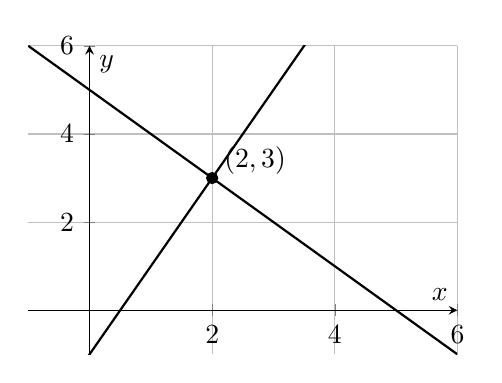
\begin{tikzpicture}
\begin{axis}[
    width=0.58\textwidth,
    height=5.5cm,
    axis lines=middle,
    xmin=-1,xmax=6,
    ymin=-1,ymax=6,
    xlabel={$x$},
    ylabel={$y$},
    grid=both,
    samples=2
]
\addplot[domain=-1:6,thick] {5-x};
\addplot[domain=-1:6,thick] {2*x-1};
\addplot[only marks,mark=*] coordinates {(2,3)};
\node at (axis cs:2.7,3.4) {\((2,3)\)};
\end{axis}
\end{tikzpicture}
\end{center}

The intersection point is the solution.

%%%%%%%%%%%%%%%%%%%%%%%%%%%%%%%%%%%%%%%%%%%%%%%%%%%%%%%%%%%%
\subsection{Three Geometric Possibilities}
\label{subsec:three-system-cases}
%%%%%%%%%%%%%%%%%%%%%%%%%%%%%%%%%%%%%%%%%%%%%%%%%%%%%%%%%%%%

Two linear equations in two variables may produce three fundamental cases.

\begin{center}
\begin{minipage}{0.31\textwidth}
\centering
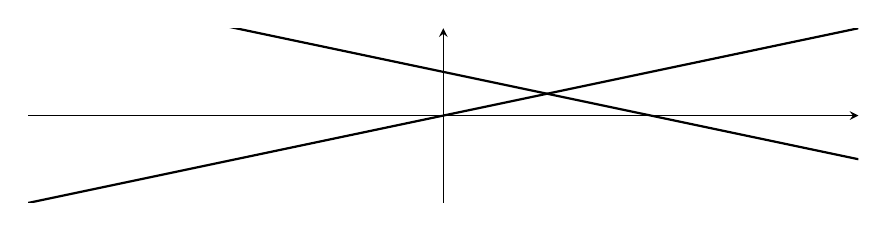
\begin{tikzpicture}
\begin{axis}[
    width=\linewidth,
    height=3.8cm,
    axis lines=middle,
    xmin=-2,xmax=2,
    ymin=-2,ymax=2,
    ticks=none
]
\addplot[domain=-2:2,thick] {x};
\addplot[domain=-2:2,thick] {-x+1};
\end{axis}
\end{tikzpicture}

One solution
\end{minipage}
\hfill
\begin{minipage}{0.31\textwidth}
\centering
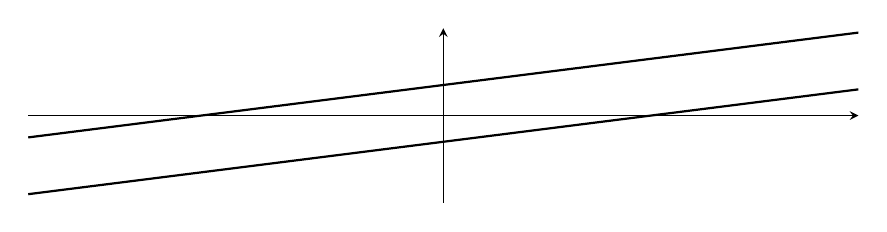
\begin{tikzpicture}
\begin{axis}[
    width=\linewidth,
    height=3.8cm,
    axis lines=middle,
    xmin=-2,xmax=2,
    ymin=-2,ymax=2,
    ticks=none
]
\addplot[domain=-2:2,thick] {0.6*x+0.7};
\addplot[domain=-2:2,thick] {0.6*x-0.6};
\end{axis}
\end{tikzpicture}

No solution
\end{minipage}
\hfill
\begin{minipage}{0.31\textwidth}
\centering
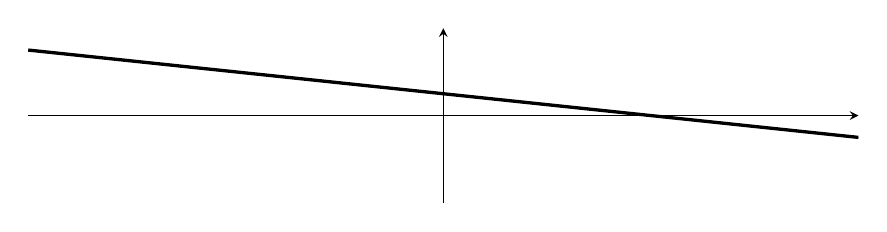
\begin{tikzpicture}
\begin{axis}[
    width=\linewidth,
    height=3.8cm,
    axis lines=middle,
    xmin=-2,xmax=2,
    ymin=-2,ymax=2,
    ticks=none
]
\addplot[domain=-2:2,very thick] {-0.5*x+0.5};
\addplot[domain=-2:2,dashed] {-0.5*x+0.5};
\end{axis}
\end{tikzpicture}

Infinitely many
\end{minipage}
\end{center}

%%%%%%%%%%%%%%%%%%%%%%%%%%%%%%%%%%%%%%%%%%%%%%%%%%%%%%%%%%%%
\subsection{Consistent and Inconsistent Systems}
\label{subsec:consistent-inconsistent-systems}
%%%%%%%%%%%%%%%%%%%%%%%%%%%%%%%%%%%%%%%%%%%%%%%%%%%%%%%%%%%%

\begin{definitionbox}{Consistent System}
A system is \emph{consistent} if it has at least one solution.
\end{definitionbox}

\begin{definitionbox}{Inconsistent System}
A system is \emph{inconsistent} if it has no solutions.
\end{definitionbox}

A consistent linear system may have exactly one solution or infinitely many
solutions.

%%%%%%%%%%%%%%%%%%%%%%%%%%%%%%%%%%%%%%%%%%%%%%%%%%%%%%%%%%%%
\subsection{Elimination}
\label{subsec:linear-elimination}
%%%%%%%%%%%%%%%%%%%%%%%%%%%%%%%%%%%%%%%%%%%%%%%%%%%%%%%%%%%%

Consider

\[ \begin{cases} x+y=5,\\ 2x-y=1. \end{cases} \]

Add the equations:

\[ 3x=6. \]

Thus,

\[ x=2. \]

Substitution gives

\[ y=3. \]

%%%%%%%%%%%%%%%%%%%%%%%%%%%%%%%%%%%%%%%%%%%%%%%%%%%%%%%%%%%%
\subsection{Worked Example: Elimination}
\label{subsec:worked-linear-system}
%%%%%%%%%%%%%%%%%%%%%%%%%%%%%%%%%%%%%%%%%%%%%%%%%%%%%%%%%%%%

\begin{workedexamplebox}{Solve a System by Elimination}

Solve

\[ \begin{cases} 2x+3y=12,\\ x-y=1. \end{cases} \]

\begin{tabularx}{\textwidth}{@{}>{\raggedright\arraybackslash}p{0.42\textwidth}X@{}}
Multiply the second equation by \(-2\). & \(-2x+2y=-2\)\\
Add the equations. & \(5y=10\)\\
Solve for \(y\). & \(y=2\)\\
Substitute into \(x-y=1\). & \(x=3\)
\end{tabularx}

\begin{answerbox}
\[ (x,y)=(3,2) \]
\end{answerbox}
\end{workedexamplebox}

%%%%%%%%%%%%%%%%%%%%%%%%%%%%%%%%%%%%%%%%%%%%%%%%%%%%%%%%%%%%
\subsection{Matrices}
\label{subsec:matrices}
%%%%%%%%%%%%%%%%%%%%%%%%%%%%%%%%%%%%%%%%%%%%%%%%%%%%%%%%%%%%

\begin{definitionbox}{Matrix}
A \emph{matrix} is a rectangular arrangement of numbers or other mathematical
objects organized into rows and columns.
\end{definitionbox}

For example,

\[ A=\begin{bmatrix}1&2&3\\4&5&6\end{bmatrix}. \]

This matrix has size

\[ 2\times3, \]

read ``two by three.''

%%%%%%%%%%%%%%%%%%%%%%%%%%%%%%%%%%%%%%%%%%%%%%%%%%%%%%%%%%%%
\subsection{Visual Structure of a Matrix}
\label{subsec:visual-matrix-structure}
%%%%%%%%%%%%%%%%%%%%%%%%%%%%%%%%%%%%%%%%%%%%%%%%%%%%%%%%%%%%

\begin{center}
\begin{tikzpicture}[every node/.style={font=\small}]
\node at (0,0) {$
A=
\begin{bmatrix}
a_{11}&a_{12}&a_{13}\\
a_{21}&a_{22}&a_{23}
\end{bmatrix}
$};

\draw[->] (-0.2,1.1) -- (-0.2,0.45);
\node at (-0.2,1.35) {column \(1\)};

\draw[->] (-1.9,-1.05) -- (-1.25,-0.35);
\node at (-2.5,-1.3) {row \(2\)};
\end{tikzpicture}
\end{center}

The entry

\[ a_{ij} \]

lies in row \(i\), column \(j\).

It is read ``\(a\) sub \(i,j\).''

%%%%%%%%%%%%%%%%%%%%%%%%%%%%%%%%%%%%%%%%%%%%%%%%%%%%%%%%%%%%
\subsection{Coefficient and Augmented Matrices}
\label{subsec:coefficient-augmented-matrices}
%%%%%%%%%%%%%%%%%%%%%%%%%%%%%%%%%%%%%%%%%%%%%%%%%%%%%%%%%%%%

The system

\[ \begin{cases} 2x+y=5,\\ 3x-4y=7 \end{cases} \]

has coefficient matrix

\[ A=\begin{bmatrix}2&1\\3&-4\end{bmatrix}. \]

The constants are

\[ \vect{b}=\begin{bmatrix}5\\7\end{bmatrix}. \]

The augmented matrix is

\[ \left[\begin{array}{cc|c}2&1&5\\3&-4&7\end{array}\right]. \]

%%%%%%%%%%%%%%%%%%%%%%%%%%%%%%%%%%%%%%%%%%%%%%%%%%%%%%%%%%%%
\subsection{From Equations to a Matrix}
\label{subsec:equations-to-matrix-visual}
%%%%%%%%%%%%%%%%%%%%%%%%%%%%%%%%%%%%%%%%%%%%%%%%%%%%%%%%%%%%

\begin{center}
\begin{tikzpicture}[
    box/.style={draw,rounded corners,align=center,inner sep=5pt},
    >=stealth
]
\node[box] (sys) at (0,0) {$
\begin{cases}
2x+y=5\\
3x-4y=7
\end{cases}
$};

\node[box] (mat) at (5,0) {$
\left[
\begin{array}{cc|c}
2&1&5\\
3&-4&7
\end{array}
\right]
$};

\draw[->,thick] (sys)--node[above]{record coefficients}(mat);
\end{tikzpicture}
\end{center}

The matrix stores the numerical structure while omitting repeated variable
symbols.

%%%%%%%%%%%%%%%%%%%%%%%%%%%%%%%%%%%%%%%%%%%%%%%%%%%%%%%%%%%%
\subsection{Elementary Row Operations}
\label{subsec:elementary-row-operations}
%%%%%%%%%%%%%%%%%%%%%%%%%%%%%%%%%%%%%%%%%%%%%%%%%%%%%%%%%%%%

The three elementary row operations are:

\begin{enumerate}
    \item interchange two rows;
    \item multiply a row by a nonzero scalar;
    \item add a scalar multiple of one row to another.
\end{enumerate}

They preserve the solution set of the associated linear system.

%%%%%%%%%%%%%%%%%%%%%%%%%%%%%%%%%%%%%%%%%%%%%%%%%%%%%%%%%%%%
\subsection{Row-Operation Notation}
\label{subsec:row-operation-notation}
%%%%%%%%%%%%%%%%%%%%%%%%%%%%%%%%%%%%%%%%%%%%%%%%%%%%%%%%%%%%

The notation

\[ R_1\leftrightarrow R_2 \]

means ``interchange rows \(1\) and \(2\).''

The notation

\[ R_2\leftarrow R_2-3R_1 \]

means

\begin{center}
``replace row \(2\) by row \(2\) minus three times row \(1\).''
\end{center}

%%%%%%%%%%%%%%%%%%%%%%%%%%%%%%%%%%%%%%%%%%%%%%%%%%%%%%%%%%%%
\subsection{Gaussian Elimination}
\label{subsec:gaussian-elimination}
%%%%%%%%%%%%%%%%%%%%%%%%%%%%%%%%%%%%%%%%%%%%%%%%%%%%%%%%%%%%

Gaussian elimination transforms a system into a simpler equivalent system.

The structural goal is

\begin{center}

\begin{tikzpicture}[
    box/.style={draw,rounded corners,inner sep=5pt},
    >=stealth
]
\node[box] (a) at (0,0) {Original matrix};
\node[box] (b) at (3.7,0) {Echelon form};
\node[box] (c) at (7.4,0) {Solve};

\draw[->,thick] (a)--node[above]{row operations}(b);
\draw[->,thick] (b)--node[above]{back substitution}(c);
\end{tikzpicture}
\end{center}

%%%%%%%%%%%%%%%%%%%%%%%%%%%%%%%%%%%%%%%%%%%%%%%%%%%%%%%%%%%%
\subsection{Row-Echelon Form}
\label{subsec:row-echelon-form}
%%%%%%%%%%%%%%%%%%%%%%%%%%%%%%%%%%%%%%%%%%%%%%%%%%%%%%%%%%%%

\begin{definitionbox}{Row-Echelon Form}
A matrix is in row-echelon form if:
\begin{enumerate}
    \item all zero rows lie below all nonzero rows;
    \item each leading entry lies to the right of the leading entry above it;
    \item all entries below each leading entry are zero.
\end{enumerate}
\end{definitionbox}

Example:

\[ \begin{bmatrix}
1&2&-1&3\\
0&1&4&2\\
0&0&5&7
\end{bmatrix}. \]

The leading entries form a staircase pattern.

%%%%%%%%%%%%%%%%%%%%%%%%%%%%%%%%%%%%%%%%%%%%%%%%%%%%%%%%%%%%
\subsection{Pivot Positions}
\label{subsec:pivot-positions}
%%%%%%%%%%%%%%%%%%%%%%%%%%%%%%%%%%%%%%%%%%%%%%%%%%%%%%%%%%%%

The location of a leading entry is a \emph{pivot position}.

For example,

\[
\begin{bmatrix}
\boxed{1}&2&5&0\\
0&\boxed{1}&-3&4\\
0&0&0&\boxed{1}
\end{bmatrix}.
\]

The corresponding columns are pivot columns.

%%%%%%%%%%%%%%%%%%%%%%%%%%%%%%%%%%%%%%%%%%%%%%%%%%%%%%%%%%%%
\subsection{Reduced Row-Echelon Form}
\label{subsec:reduced-row-echelon-form}
%%%%%%%%%%%%%%%%%%%%%%%%%%%%%%%%%%%%%%%%%%%%%%%%%%%%%%%%%%%%

\begin{definitionbox}{Reduced Row-Echelon Form}
A matrix is in reduced row-echelon form if:
\begin{enumerate}
    \item it is in row-echelon form;
    \item each leading entry is \(1\);
    \item each leading \(1\) is the only nonzero entry in its column.
\end{enumerate}
\end{definitionbox}

Reduced row-echelon form is abbreviated \emph{RREF}.

%%%%%%%%%%%%%%%%%%%%%%%%%%%%%%%%%%%%%%%%%%%%%%%%%%%%%%%%%%%%
\subsection{Worked Example: Row Reduction}
\label{subsec:worked-row-reduction}
%%%%%%%%%%%%%%%%%%%%%%%%%%%%%%%%%%%%%%%%%%%%%%%%%%%%%%%%%%%%

\begin{workedexamplebox}{Solve a System by Row Reduction}

Solve

\[ \begin{cases}
x+y+z=6,\\
2x-y+z=3,\\
x+2y-z=2.
\end{cases} \]

Start with

\[ \left[\begin{array}{ccc|c}
1&1&1&6\\
2&-1&1&3\\
1&2&-1&2
\end{array}\right]. \]

\begin{tabularx}{\textwidth}{@{}>{\raggedright\arraybackslash}p{0.42\textwidth}X@{}}
\(R_2\leftarrow R_2-2R_1\). &
\(\left[\begin{array}{ccc|c}
1&1&1&6\\0&-3&-1&-9\\1&2&-1&2
\end{array}\right]\)\\[3mm]
\(R_3\leftarrow R_3-R_1\). &
\(\left[\begin{array}{ccc|c}
1&1&1&6\\0&-3&-1&-9\\0&1&-2&-4
\end{array}\right]\)\\[3mm]
Interchange \(R_2,R_3\). &
\(\left[\begin{array}{ccc|c}
1&1&1&6\\0&1&-2&-4\\0&-3&-1&-9
\end{array}\right]\)\\[3mm]
\(R_3\leftarrow R_3+3R_2\). &
\(\left[\begin{array}{ccc|c}
1&1&1&6\\0&1&-2&-4\\0&0&-7&-21
\end{array}\right]\)
\end{tabularx}

Back substitution gives

\[ z=3,\qquad y=2,\qquad x=1. \]

\begin{answerbox}
\[ (x,y,z)=(1,2,3) \]
\end{answerbox}
\end{workedexamplebox}

%%%%%%%%%%%%%%%%%%%%%%%%%%%%%%%%%%%%%%%%%%%%%%%%%%%%%%%%%%%%
\subsection{Free Variables}
\label{subsec:free-variables}
%%%%%%%%%%%%%%%%%%%%%%%%%%%%%%%%%%%%%%%%%%%%%%%%%%%%%%%%%%%%

Suppose RREF gives

\[ \left[\begin{array}{ccc|c}
1&2&0&4\\
0&0&1&3
\end{array}\right]. \]

Then \(x_1,x_3\) are basic variables and \(x_2\) is free.

Let

\[ x_2=t. \]

Then

\[ x_1=4-2t,\qquad x_3=3. \]

%%%%%%%%%%%%%%%%%%%%%%%%%%%%%%%%%%%%%%%%%%%%%%%%%%%%%%%%%%%%
\subsection{Parametric Vector Form}
\label{subsec:parametric-vector-form}
%%%%%%%%%%%%%%%%%%%%%%%%%%%%%%%%%%%%%%%%%%%%%%%%%%%%%%%%%%%%

The solution can be written

\[ \begin{bmatrix}x_1\\x_2\\x_3\end{bmatrix}
=
\begin{bmatrix}4\\0\\3\end{bmatrix}
+t
\begin{bmatrix}-2\\1\\0\end{bmatrix}. \]

Geometrically, this describes a line in \(\R^3\).

\begin{center}
\begin{tikzpicture}[scale=0.9,>=stealth]
\draw[->] (-0.5,0)--(5,0) node[right]{\(x\)};
\draw[->] (0,-0.5)--(0,4) node[above]{\(y\)};
\draw[thick] (0.8,0.8)--(4.4,3.2);
\fill (1.5,1.27) circle (2pt);
\node[above left] at (1.5,1.27) {\(\vect{p}\)};
\draw[->,very thick] (1.5,1.27)--(3,2.27);
\node[right] at (3,2.27) {\(\vect{v}\)};
\end{tikzpicture}
\end{center}

The general structure is

\[ \vect{x}=\vect{p}+t\vect{v}. \]

%%%%%%%%%%%%%%%%%%%%%%%%%%%%%%%%%%%%%%%%%%%%%%%%%%%%%%%%%%%%
\subsection{Detecting Inconsistency}
\label{subsec:detecting-inconsistency}
%%%%%%%%%%%%%%%%%%%%%%%%%%%%%%%%%%%%%%%%%%%%%%%%%%%%%%%%%%%%

A row such as

\[ \left[\begin{array}{ccc|c}0&0&0&5\end{array}\right] \]

represents

\[ 0=5. \]

This is impossible.

Therefore the system is inconsistent.

%%%%%%%%%%%%%%%%%%%%%%%%%%%%%%%%%%%%%%%%%%%%%%%%%%%%%%%%%%%%
\subsection{Homogeneous Systems}
\label{subsec:homogeneous-systems}
%%%%%%%%%%%%%%%%%%%%%%%%%%%%%%%%%%%%%%%%%%%%%%%%%%%%%%%%%%%%

\begin{definitionbox}{Homogeneous Linear System}
A homogeneous linear system has the form
\[ A\vect{x}=\zero. \]
\end{definitionbox}

The zero vector is always a solution.

It is called the \emph{trivial solution}.

Any nonzero solution is called a \emph{nontrivial solution}.

%%%%%%%%%%%%%%%%%%%%%%%%%%%%%%%%%%%%%%%%%%%%%%%%%%%%%%%%%%%%
\subsection{Matrix Addition and Scalar Multiplication}
\label{subsec:matrix-addition-scalar}
%%%%%%%%%%%%%%%%%%%%%%%%%%%%%%%%%%%%%%%%%%%%%%%%%%%%%%%%%%%%

Matrices of the same size are added entrywise.

\[ \begin{bmatrix}1&2\\3&4\end{bmatrix}
+\begin{bmatrix}5&-1\\2&0\end{bmatrix}
=
\begin{bmatrix}6&1\\5&4\end{bmatrix}. \]

Scalar multiplication also acts entrywise:

\[ 3\begin{bmatrix}1&-2\\4&5\end{bmatrix}
=
\begin{bmatrix}3&-6\\12&15\end{bmatrix}. \]

%%%%%%%%%%%%%%%%%%%%%%%%%%%%%%%%%%%%%%%%%%%%%%%%%%%%%%%%%%%%
\subsection{Matrix Multiplication}
\label{subsec:matrix-multiplication}
%%%%%%%%%%%%%%%%%%%%%%%%%%%%%%%%%%%%%%%%%%%%%%%%%%%%%%%%%%%%

If \(A\) is \(m\times n\) and \(B\) is \(n\times p\), then

\[ AB \]

is defined and has size

\[ m\times p. \]

The inner dimensions must agree.

%%%%%%%%%%%%%%%%%%%%%%%%%%%%%%%%%%%%%%%%%%%%%%%%%%%%%%%%%%%%
\subsection{Visual Rule for Matrix Dimensions}
\label{subsec:matrix-dimension-visual}
%%%%%%%%%%%%%%%%%%%%%%%%%%%%%%%%%%%%%%%%%%%%%%%%%%%%%%%%%%%%

\begin{center}
\[
\underbrace{A}_{m\times\boxed{n}}
\;
\underbrace{B}_{\boxed{n}\times p}
\quad\Longrightarrow\quad
\underbrace{AB}_{m\times p}.
\]
\end{center}

The matching inner dimensions disappear, leaving the outer dimensions.

%%%%%%%%%%%%%%%%%%%%%%%%%%%%%%%%%%%%%%%%%%%%%%%%%%%%%%%%%%%%
\subsection{Row-by-Column Multiplication}
\label{subsec:row-column-multiplication}
%%%%%%%%%%%%%%%%%%%%%%%%%%%%%%%%%%%%%%%%%%%%%%%%%%%%%%%%%%%%

If

\[ C=AB, \]

then

\[ c_{ij}=\sum_{k=1}^{n}a_{ik}b_{kj}. \]

The symbol

\[ \sum \]

is the summation symbol and is read ``the sum.''

Thus

\[ \sum_{k=1}^{n}a_{ik}b_{kj} \]

means

\begin{center}
``the sum from \(k=1\) to \(n\) of \(a_{ik}b_{kj}\).''
\end{center}

%%%%%%%%%%%%%%%%%%%%%%%%%%%%%%%%%%%%%%%%%%%%%%%%%%%%%%%%%%%%
\subsection{Visual Matrix Product}
\label{subsec:visual-matrix-product}
%%%%%%%%%%%%%%%%%%%%%%%%%%%%%%%%%%%%%%%%%%%%%%%%%%%%%%%%%%%%

\begin{center}
\begin{tikzpicture}[every node/.style={font=\small}]
\node at (0,0) {$
\begin{bmatrix}
\boxed{a_{11}}&\boxed{a_{12}}\\
a_{21}&a_{22}
\end{bmatrix}
$};

\node at (3,0) {$
\begin{bmatrix}
\boxed{b_{11}}&b_{12}\\
\boxed{b_{21}}&b_{22}
\end{bmatrix}
$};

\node at (6,0) {$
\begin{bmatrix}
\boxed{a_{11}b_{11}+a_{12}b_{21}}&\cdots\\
\cdots&\cdots
\end{bmatrix}
$};

\node at (1.5,0) {\(\times\)};
\node at (4.5,0) {\(=\)};
\end{tikzpicture}
\end{center}

A row of the first matrix combines with a column of the second.

%%%%%%%%%%%%%%%%%%%%%%%%%%%%%%%%%%%%%%%%%%%%%%%%%%%%%%%%%%%%
\subsection{Worked Example: Matrix Multiplication}
\label{subsec:worked-matrix-multiplication}
%%%%%%%%%%%%%%%%%%%%%%%%%%%%%%%%%%%%%%%%%%%%%%%%%%%%%%%%%%%%

\begin{workedexamplebox}{Multiply Two Matrices}

Let

\[ A=\begin{bmatrix}1&2\\3&4\end{bmatrix},\qquad
B=\begin{bmatrix}5&6\\7&8\end{bmatrix}. \]

\begin{tabularx}{\textwidth}{@{}>{\raggedright\arraybackslash}p{0.42\textwidth}X@{}}
First row, first column. & \(1(5)+2(7)=19\)\\
First row, second column. & \(1(6)+2(8)=22\)\\
Second row, first column. & \(3(5)+4(7)=43\)\\
Second row, second column. & \(3(6)+4(8)=50\)
\end{tabularx}

\begin{answerbox}
\[ AB=\begin{bmatrix}19&22\\43&50\end{bmatrix} \]
\end{answerbox}
\end{workedexamplebox}

%%%%%%%%%%%%%%%%%%%%%%%%%%%%%%%%%%%%%%%%%%%%%%%%%%%%%%%%%%%%
\subsection{Matrix Multiplication Is Not Commutative}
\label{subsec:matrix-not-commutative}
%%%%%%%%%%%%%%%%%%%%%%%%%%%%%%%%%%%%%%%%%%%%%%%%%%%%%%%%%%%%

In general,

\[ AB\neq BA. \]

Matrix multiplication is associative:

\[ A(BC)=(AB)C, \]

and distributive:

\[ A(B+C)=AB+AC. \]

But order matters.

%%%%%%%%%%%%%%%%%%%%%%%%%%%%%%%%%%%%%%%%%%%%%%%%%%%%%%%%%%%%
\subsection{Identity Matrix}
\label{subsec:identity-matrix}
%%%%%%%%%%%%%%%%%%%%%%%%%%%%%%%%%%%%%%%%%%%%%%%%%%%%%%%%%%%%

\begin{definitionbox}{Identity Matrix}
The identity matrix \(I_n\) is the \(n\times n\) matrix with \(1\)'s on the
main diagonal and \(0\)'s elsewhere.
\end{definitionbox}

For example,

\[ I_3=\begin{bmatrix}1&0&0\\0&1&0\\0&0&1\end{bmatrix}. \]

For compatible \(A\),

\[ AI=IA=A. \]

%%%%%%%%%%%%%%%%%%%%%%%%%%%%%%%%%%%%%%%%%%%%%%%%%%%%%%%%%%%%
\subsection{Transpose}
\label{subsec:matrix-transpose}
%%%%%%%%%%%%%%%%%%%%%%%%%%%%%%%%%%%%%%%%%%%%%%%%%%%%%%%%%%%%

The transpose of \(A\), written

\[ A^{\mathsf T}, \]

interchanges rows and columns.

For example,

\[ \begin{bmatrix}1&2&3\\4&5&6\end{bmatrix}^{\mathsf T}
=
\begin{bmatrix}1&4\\2&5\\3&6\end{bmatrix}. \]

%%%%%%%%%%%%%%%%%%%%%%%%%%%%%%%%%%%%%%%%%%%%%%%%%%%%%%%%%%%%
\subsection{Inverse Matrices}
\label{subsec:inverse-matrices}
%%%%%%%%%%%%%%%%%%%%%%%%%%%%%%%%%%%%%%%%%%%%%%%%%%%%%%%%%%%%

\begin{definitionbox}{Inverse Matrix}
A square matrix \(A\) is invertible if there exists \(A^{-1}\) such that
\[ AA^{-1}=A^{-1}A=I. \]
\end{definitionbox}

The notation

\[ A^{-1} \]

is read ``\(A\) inverse.''

%%%%%%%%%%%%%%%%%%%%%%%%%%%%%%%%%%%%%%%%%%%%%%%%%%%%%%%%%%%%
\subsection{Solving Systems Using an Inverse}
\label{subsec:systems-inverse}
%%%%%%%%%%%%%%%%%%%%%%%%%%%%%%%%%%%%%%%%%%%%%%%%%%%%%%%%%%%%

Suppose

\[ A\vect{x}=\vect{b}. \]

If \(A\) is invertible,

\[ A^{-1}A\vect{x}=A^{-1}\vect{b}, \]

so

\[ \vect{x}=A^{-1}\vect{b}. \]

%%%%%%%%%%%%%%%%%%%%%%%%%%%%%%%%%%%%%%%%%%%%%%%%%%%%%%%%%%%%
\subsection{Determinants}
\label{subsec:determinants}
%%%%%%%%%%%%%%%%%%%%%%%%%%%%%%%%%%%%%%%%%%%%%%%%%%%%%%%%%%%%

\begin{definitionbox}{Determinant}
The determinant is a scalar associated with a square matrix that records
information about invertibility, scaling, and orientation.
\end{definitionbox}

It is written

\[ \det(A). \]

For

\[ A=\begin{bmatrix}a&b\\c&d\end{bmatrix}, \]

\[ \det(A)=ad-bc. \]

%%%%%%%%%%%%%%%%%%%%%%%%%%%%%%%%%%%%%%%%%%%%%%%%%%%%%%%%%%%%
\subsection{Determinant as Area}
\label{subsec:determinant-area}
%%%%%%%%%%%%%%%%%%%%%%%%%%%%%%%%%%%%%%%%%%%%%%%%%%%%%%%%%%%%

Consider two vectors

\[ \vect{u}=\begin{bmatrix}u_1\\u_2\end{bmatrix},\qquad
\vect{v}=\begin{bmatrix}v_1\\v_2\end{bmatrix}. \]

They determine a parallelogram.

\begin{center}
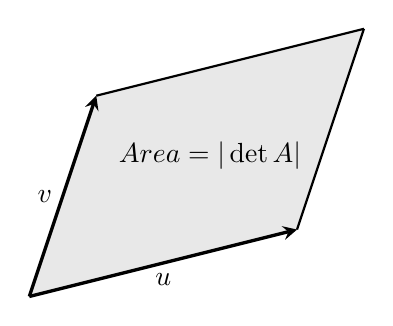
\begin{tikzpicture}[scale=0.85,>=stealth]
\coordinate (O) at (0,0);
\coordinate (U) at (4,1);
\coordinate (V) at (1,3);
\coordinate (UV) at (5,4);

\fill[gray!18] (O)--(U)--(UV)--(V)--cycle;

\draw[->,very thick] (O)--(U)
    node[midway,below] {\(\vect{u}\)};

\draw[->,very thick] (O)--(V)
    node[midway,left] {\(\vect{v}\)};

\draw[thick] (U)--(UV);
\draw[thick] (V)--(UV);

\node at (2.7,2.1) {\(\text{Area}=|\det A|\)};
\end{tikzpicture}
\end{center}

If

\[ A=\begin{bmatrix}u_1&v_1\\u_2&v_2\end{bmatrix}, \]

then the parallelogram area is

\[ |\det(A)|. \]

%%%%%%%%%%%%%%%%%%%%%%%%%%%%%%%%%%%%%%%%%%%%%%%%%%%%%%%%%%%%
\subsection{Determinant and Linear Dependence}
\label{subsec:determinant-dependence}
%%%%%%%%%%%%%%%%%%%%%%%%%%%%%%%%%%%%%%%%%%%%%%%%%%%%%%%%%%%%

If the column vectors are parallel, the parallelogram collapses to a line.

\begin{center}
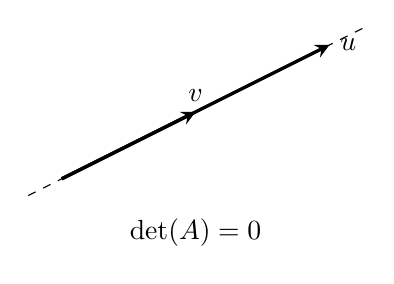
\begin{tikzpicture}[scale=0.85,>=stealth]
\draw[->,very thick] (0,0)--(4,2) node[right]{\(\vect{u}\)};
\draw[->,very thick] (0,0)--(2,1) node[above]{\(\vect{v}\)};
\draw[dashed] (-0.5,-0.25)--(4.5,2.25);
\node at (2,-0.8) {\(\det(A)=0\)};
\end{tikzpicture}
\end{center}

Therefore,

\[ \det(A)=0 \]

indicates linear dependence for a square matrix.

%%%%%%%%%%%%%%%%%%%%%%%%%%%%%%%%%%%%%%%%%%%%%%%%%%%%%%%%%%%%
\subsection{Determinant and Invertibility}
\label{subsec:determinant-invertibility}
%%%%%%%%%%%%%%%%%%%%%%%%%%%%%%%%%%%%%%%%%%%%%%%%%%%%%%%%%%%%

A square matrix is invertible if and only if

\[ \det(A)\neq0. \]

If

\[ \det(A)=0, \]

the transformation collapses at least one dimension and cannot be reversed.

%%%%%%%%%%%%%%%%%%%%%%%%%%%%%%%%%%%%%%%%%%%%%%%%%%%%%%%%%%%%
\subsection{Vectors}
\label{subsec:vectors}
%%%%%%%%%%%%%%%%%%%%%%%%%%%%%%%%%%%%%%%%%%%%%%%%%%%%%%%%%%%%

A vector in \(\R^n\) may be written

\[ \vect{v}=\begin{bmatrix}v_1\\v_2\\\vdots\\v_n\end{bmatrix}. \]

In \(\R^2\) and \(\R^3\), vectors may be visualized as directed line segments.

\begin{center}
\begin{tikzpicture}[scale=0.85,>=stealth]
\draw[->] (-0.5,0)--(5,0) node[right]{\(x\)};
\draw[->] (0,-0.5)--(0,4) node[above]{\(y\)};
\draw[->,very thick] (0,0)--(4,3) node[right]{\(\vect{v}\)};
\draw[dashed] (4,0)--(4,3);
\draw[dashed] (0,3)--(4,3);
\node[below] at (4,0) {\(v_1\)};
\node[left] at (0,3) {\(v_2\)};
\end{tikzpicture}
\end{center}

%%%%%%%%%%%%%%%%%%%%%%%%%%%%%%%%%%%%%%%%%%%%%%%%%%%%%%%%%%%%
\subsection{Vector Addition}
\label{subsec:vector-addition}
%%%%%%%%%%%%%%%%%%%%%%%%%%%%%%%%%%%%%%%%%%%%%%%%%%%%%%%%%%%%

Vectors are added componentwise.

\[ \begin{bmatrix}1\\2\end{bmatrix}
+\begin{bmatrix}3\\1\end{bmatrix}
=
\begin{bmatrix}4\\3\end{bmatrix}. \]

Geometrically, vector addition follows the tip-to-tail rule.

\begin{center}
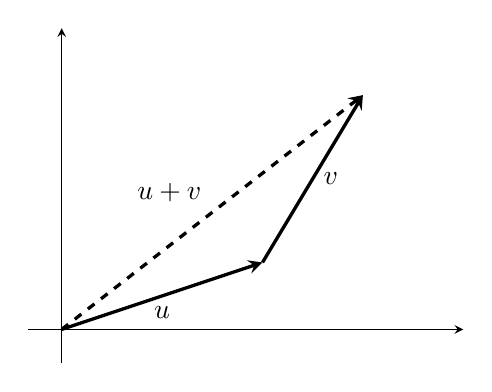
\begin{tikzpicture}[scale=0.85,>=stealth]
\draw[->] (-0.5,0)--(6,0);
\draw[->] (0,-0.5)--(0,4.5);

\draw[->,very thick] (0,0)--(3,1)
    node[midway,below]{\(\vect{u}\)};

\draw[->,very thick] (3,1)--(4.5,3.5)
    node[midway,right]{\(\vect{v}\)};

\draw[->,very thick,dashed] (0,0)--(4.5,3.5)
    node[midway,above left]{\(\vect{u}+\vect{v}\)};
\end{tikzpicture}
\end{center}

%%%%%%%%%%%%%%%%%%%%%%%%%%%%%%%%%%%%%%%%%%%%%%%%%%%%%%%%%%%%
\subsection{Scalar Multiplication}
\label{subsec:vector-scalar-multiplication}
%%%%%%%%%%%%%%%%%%%%%%%%%%%%%%%%%%%%%%%%%%%%%%%%%%%%%%%%%%%%

Scalar multiplication changes a vector's magnitude and possibly its direction.

\begin{center}
\begin{tikzpicture}[scale=0.8,>=stealth]
\draw[->] (-4,0)--(6,0);
\draw[->] (0,-1)--(0,4);

\draw[->,very thick] (0,0)--(2,1)
node[right]{\(\vect{v}\)};

\draw[->,very thick] (0,0)--(4,2)
node[right]{\(2\vect{v}\)};

\draw[->,very thick] (0,0)--(-2,-1)
node[left]{\(-\vect{v}\)};
\end{tikzpicture}
\end{center}

Positive scalars preserve direction.

Negative scalars reverse direction.

%%%%%%%%%%%%%%%%%%%%%%%%%%%%%%%%%%%%%%%%%%%%%%%%%%%%%%%%%%%%
\subsection{Linear Combinations}
\label{subsec:linear-combinations}
%%%%%%%%%%%%%%%%%%%%%%%%%%%%%%%%%%%%%%%%%%%%%%%%%%%%%%%%%%%%

\begin{definitionbox}{Linear Combination}
A linear combination of vectors
\(\vect{v}_1,\ldots,\vect{v}_k\) is
\[ c_1\vect{v}_1+\cdots+c_k\vect{v}_k, \]
where \(c_1,\ldots,c_k\) are scalars.
\end{definitionbox}

%%%%%%%%%%%%%%%%%%%%%%%%%%%%%%%%%%%%%%%%%%%%%%%%%%%%%%%%%%%%
\subsection{Span}
\label{subsec:span}
%%%%%%%%%%%%%%%%%%%%%%%%%%%%%%%%%%%%%%%%%%%%%%%%%%%%%%%%%%%%

\begin{definitionbox}{Span}
The span of vectors
\(\vect{v}_1,\ldots,\vect{v}_k\) is the set of all their linear combinations.
\end{definitionbox}

It is written

\[ \Span\{\vect{v}_1,\ldots,\vect{v}_k\}. \]

%%%%%%%%%%%%%%%%%%%%%%%%%%%%%%%%%%%%%%%%%%%%%%%%%%%%%%%%%%%%
\subsection{One Vector Spans a Line}
\label{subsec:one-vector-span}
%%%%%%%%%%%%%%%%%%%%%%%%%%%%%%%%%%%%%%%%%%%%%%%%%%%%%%%%%%%%

For a nonzero vector \(\vect{v}\in\R^2\),

\[ \Span\{\vect{v}\}=\{c\vect{v}:c\in\R\}. \]

Geometrically this is a line through the origin.

\begin{center}
\begin{tikzpicture}[scale=0.85,>=stealth]
\draw[->] (-4,0)--(5,0);
\draw[->] (0,-3)--(0,4);

\draw[thick] (-3,-2)--(4.5,3);
\draw[->,very thick] (0,0)--(2.4,1.6)
node[right]{\(\vect{v}\)};

\node at (-2.5,2.2) {\(\Span\{\vect{v}\}\)};
\end{tikzpicture}
\end{center}

%%%%%%%%%%%%%%%%%%%%%%%%%%%%%%%%%%%%%%%%%%%%%%%%%%%%%%%%%%%%
\subsection{Two Independent Vectors Span a Plane}
\label{subsec:two-vector-span}
%%%%%%%%%%%%%%%%%%%%%%%%%%%%%%%%%%%%%%%%%%%%%%%%%%%%%%%%%%%%

Two independent vectors in \(\R^2\) span the entire plane.

\begin{center}
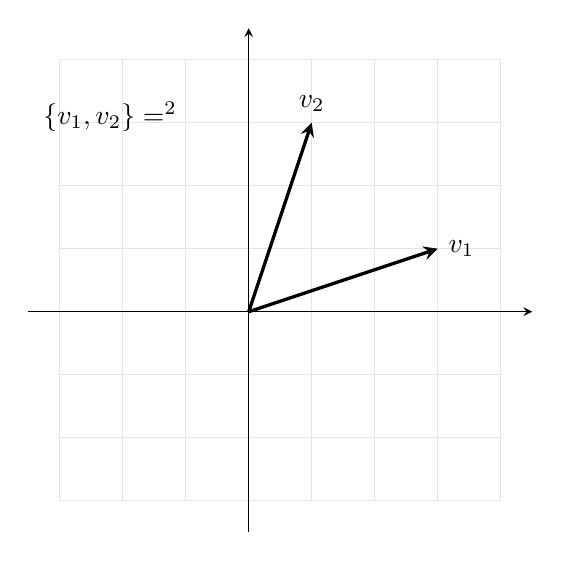
\begin{tikzpicture}[scale=0.8,>=stealth]
\draw[step=1cm,gray!20,very thin] (-3,-3) grid (4,4);
\draw[->] (-3.5,0)--(4.5,0);
\draw[->] (0,-3.5)--(0,4.5);

\draw[->,very thick] (0,0)--(3,1)
node[right]{\(\vect{v}_1\)};

\draw[->,very thick] (0,0)--(1,3)
node[above]{\(\vect{v}_2\)};

\node at (-2.2,3.1) {\(\Span\{\vect{v}_1,\vect{v}_2\}=\R^2\)};
\end{tikzpicture}
\end{center}

%%%%%%%%%%%%%%%%%%%%%%%%%%%%%%%%%%%%%%%%%%%%%%%%%%%%%%%%%%%%
\subsection{Linear Independence}
\label{subsec:linear-independence}
%%%%%%%%%%%%%%%%%%%%%%%%%%%%%%%%%%%%%%%%%%%%%%%%%%%%%%%%%%%%

\begin{definitionbox}{Linear Independence}
Vectors \(\vect{v}_1,\ldots,\vect{v}_k\) are linearly independent if
\[ c_1\vect{v}_1+\cdots+c_k\vect{v}_k=\zero \]
implies
\[ c_1=\cdots=c_k=0. \]
\end{definitionbox}

Otherwise they are linearly dependent.

%%%%%%%%%%%%%%%%%%%%%%%%%%%%%%%%%%%%%%%%%%%%%%%%%%%%%%%%%%%%
\subsection{Visualizing Independence}
\label{subsec:visualizing-independence}
%%%%%%%%%%%%%%%%%%%%%%%%%%%%%%%%%%%%%%%%%%%%%%%%%%%%%%%%%%%%

Two nonzero vectors in \(\R^2\) are independent if neither is a scalar
multiple of the other.

\begin{center}
\begin{minipage}{0.46\textwidth}
\centering
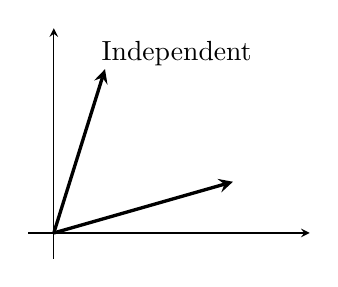
\begin{tikzpicture}[scale=0.65,>=stealth]
\draw[->] (-0.5,0)--(5,0);
\draw[->] (0,-0.5)--(0,4);
\draw[->,very thick] (0,0)--(3.5,1);
\draw[->,very thick] (0,0)--(1,3.2);
\node at (2.4,3.5) {Independent};
\end{tikzpicture}
\end{minipage}
\hfill
\begin{minipage}{0.46\textwidth}
\centering
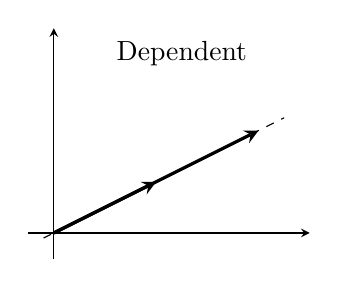
\begin{tikzpicture}[scale=0.65,>=stealth]
\draw[->] (-0.5,0)--(5,0);
\draw[->] (0,-0.5)--(0,4);
\draw[dashed] (-0.2,-0.1)--(4.5,2.25);
\draw[->,very thick] (0,0)--(2,1);
\draw[->,very thick] (0,0)--(4,2);
\node at (2.5,3.5) {Dependent};
\end{tikzpicture}
\end{minipage}
\end{center}

%%%%%%%%%%%%%%%%%%%%%%%%%%%%%%%%%%%%%%%%%%%%%%%%%%%%%%%%%%%%
\subsection{Worked Example: Linear Dependence}
\label{subsec:worked-linear-independence}
%%%%%%%%%%%%%%%%%%%%%%%%%%%%%%%%%%%%%%%%%%%%%%%%%%%%%%%%%%%%

\begin{workedexamplebox}{Determine Whether Vectors Are Independent}

Let

\[ \vect{v}_1=\begin{bmatrix}1\\2\end{bmatrix},\qquad
\vect{v}_2=\begin{bmatrix}3\\6\end{bmatrix}. \]

\begin{tabularx}{\textwidth}{@{}>{\raggedright\arraybackslash}p{0.42\textwidth}X@{}}
Compare the vectors. & \(\vect{v}_2=3\vect{v}_1\)\\
Rearrange. & \(3\vect{v}_1-\vect{v}_2=\zero\)\\
A nontrivial relation exists. & The vectors are dependent.
\end{tabularx}

\begin{answerbox}
The vectors are linearly dependent.
\end{answerbox}
\end{workedexamplebox}

%%%%%%%%%%%%%%%%%%%%%%%%%%%%%%%%%%%%%%%%%%%%%%%%%%%%%%%%%%%%
\subsection{Vector Spaces}
\label{subsec:vector-spaces}
%%%%%%%%%%%%%%%%%%%%%%%%%%%%%%%%%%%%%%%%%%%%%%%%%%%%%%%%%%%%

\begin{definitionbox}{Vector Space}
A vector space over a field \(\F\) is a set \(V\) equipped with vector addition
and scalar multiplication satisfying the vector-space axioms.
\end{definitionbox}

Examples include

\begin{itemize}
    \item \(\R^n\);
    \item \(\C^n\);
    \item matrices of a fixed size;
    \item polynomial spaces;
    \item spaces of functions;
    \item solution spaces of homogeneous differential equations.
\end{itemize}

%%%%%%%%%%%%%%%%%%%%%%%%%%%%%%%%%%%%%%%%%%%%%%%%%%%%%%%%%%%%
\subsection{Subspaces}
\label{subsec:subspaces}
%%%%%%%%%%%%%%%%%%%%%%%%%%%%%%%%%%%%%%%%%%%%%%%%%%%%%%%%%%%%

\begin{definitionbox}{Subspace}
A subset \(W\subseteq V\) is a subspace if it is itself a vector space using
the operations inherited from \(V\).
\end{definitionbox}

A useful test is:

\begin{enumerate}
    \item \(\zero\in W\);
    \item \(W\) is closed under vector addition;
    \item \(W\) is closed under scalar multiplication.
\end{enumerate}

%%%%%%%%%%%%%%%%%%%%%%%%%%%%%%%%%%%%%%%%%%%%%%%%%%%%%%%%%%%%
\subsection{Visualizing a Subspace}
\label{subsec:visual-subspace}
%%%%%%%%%%%%%%%%%%%%%%%%%%%%%%%%%%%%%%%%%%%%%%%%%%%%%%%%%%%%

A line through the origin is a subspace of \(\R^2\).

\begin{center}
\begin{tikzpicture}[scale=0.8,>=stealth]
\draw[->] (-4,0)--(5,0);
\draw[->] (0,-3)--(0,4);
\draw[very thick] (-3,-2)--(4.5,3);
\fill (0,0) circle (2pt);
\node[above left] at (0,0) {\(\zero\)};
\node at (-2.2,2.4) {\(W\)};
\end{tikzpicture}
\end{center}

A parallel line not passing through the origin is not a subspace because it
does not contain \(\zero\).

%%%%%%%%%%%%%%%%%%%%%%%%%%%%%%%%%%%%%%%%%%%%%%%%%%%%%%%%%%%%
\subsection{Worked Example: Subspace Test}
\label{subsec:worked-subspace}
%%%%%%%%%%%%%%%%%%%%%%%%%%%%%%%%%%%%%%%%%%%%%%%%%%%%%%%%%%%%

\begin{workedexamplebox}{Determine Whether a Set Is a Subspace}

Let

\[ W=\left\{\begin{bmatrix}x\\y\end{bmatrix}\in\R^2:x+y=0\right\}. \]

\begin{tabularx}{\textwidth}{@{}>{\raggedright\arraybackslash}p{0.42\textwidth}X@{}}
Zero vector. & \(0+0=0\)\\
General elements. & \(\vect{u}=(a,-a),\;\vect{v}=(b,-b)\)\\
Addition. & \(\vect{u}+\vect{v}=(a+b,-a-b)\in W\)\\
Scalar multiplication. & \(c\vect{u}=(ca,-ca)\in W\)
\end{tabularx}

\begin{answerbox}
\(W\) is a subspace of \(\R^2\).
\end{answerbox}
\end{workedexamplebox}

%%%%%%%%%%%%%%%%%%%%%%%%%%%%%%%%%%%%%%%%%%%%%%%%%%%%%%%%%%%%
\subsection{Bases}
\label{subsec:bases}
%%%%%%%%%%%%%%%%%%%%%%%%%%%%%%%%%%%%%%%%%%%%%%%%%%%%%%%%%%%%

\begin{definitionbox}{Basis}
A basis of a vector space \(V\) is a set of vectors that:
\begin{enumerate}
    \item spans \(V\);
    \item is linearly independent.
\end{enumerate}
\end{definitionbox}

The standard basis of \(\R^2\) is

\[ \vect{e}_1=\begin{bmatrix}1\\0\end{bmatrix},\qquad
\vect{e}_2=\begin{bmatrix}0\\1\end{bmatrix}. \]

%%%%%%%%%%%%%%%%%%%%%%%%%%%%%%%%%%%%%%%%%%%%%%%%%%%%%%%%%%%%
\subsection{Visualizing a Basis}
\label{subsec:visual-basis}
%%%%%%%%%%%%%%%%%%%%%%%%%%%%%%%%%%%%%%%%%%%%%%%%%%%%%%%%%%%%

\begin{center}
\begin{tikzpicture}[scale=1.0,>=stealth]
\draw[->] (-0.5,0)--(4,0) node[right]{\(x\)};
\draw[->] (0,-0.5)--(0,4) node[above]{\(y\)};

\draw[->,very thick] (0,0)--(2.5,0)
node[below]{\(\vect{e}_1\)};

\draw[->,very thick] (0,0)--(0,2.5)
node[left]{\(\vect{e}_2\)};

\draw[->,thick,dashed] (0,0)--(3,2)
node[right]{\(\vect{v}=3\vect{e}_1+2\vect{e}_2\)};

\draw[dashed] (3,0)--(3,2);
\draw[dashed] (0,2)--(3,2);
\end{tikzpicture}
\end{center}

A basis provides coordinate directions from which every vector in the space
can be constructed uniquely.

%%%%%%%%%%%%%%%%%%%%%%%%%%%%%%%%%%%%%%%%%%%%%%%%%%%%%%%%%%%%
\subsection{Coordinates Relative to a Basis}
\label{subsec:coordinates-basis}
%%%%%%%%%%%%%%%%%%%%%%%%%%%%%%%%%%%%%%%%%%%%%%%%%%%%%%%%%%%%

If

\[ \mathcal B=\{\vect{v}_1,\ldots,\vect{v}_n\} \]

is a basis, then every vector \(\vect{v}\) has a unique representation

\[ \vect{v}=c_1\vect{v}_1+\cdots+c_n\vect{v}_n. \]

Its coordinate vector relative to \(\mathcal B\) is

\[ [\vect{v}]_{\mathcal B}
=
\begin{bmatrix}c_1\\\vdots\\c_n\end{bmatrix}. \]

%%%%%%%%%%%%%%%%%%%%%%%%%%%%%%%%%%%%%%%%%%%%%%%%%%%%%%%%%%%%
\subsection{Dimension}
\label{subsec:dimension}
%%%%%%%%%%%%%%%%%%%%%%%%%%%%%%%%%%%%%%%%%%%%%%%%%%%%%%%%%%%%

\begin{definitionbox}{Dimension}
The dimension of a finite-dimensional vector space is the number of vectors
in any basis.
\end{definitionbox}

It is written

\[ \dim(V). \]

Thus,

\[ \dim(\R^2)=2,\qquad \dim(\R^3)=3. \]

%%%%%%%%%%%%%%%%%%%%%%%%%%%%%%%%%%%%%%%%%%%%%%%%%%%%%%%%%%%%
\subsection{Column Space}
\label{subsec:column-space}
%%%%%%%%%%%%%%%%%%%%%%%%%%%%%%%%%%%%%%%%%%%%%%%%%%%%%%%%%%%%

The column space of a matrix \(A\) is the span of its columns.

It is written

\[ \operatorname{Col}(A). \]

If

\[ A=\begin{bmatrix}\vert&\vert\\\vect{a}_1&\vect{a}_2\\\vert&\vert\end{bmatrix}, \]

then

\[ \operatorname{Col}(A)=\Span\{\vect{a}_1,\vect{a}_2\}. \]

%%%%%%%%%%%%%%%%%%%%%%%%%%%%%%%%%%%%%%%%%%%%%%%%%%%%%%%%%%%%
\subsection{Visualizing Column Space}
\label{subsec:visual-column-space}
%%%%%%%%%%%%%%%%%%%%%%%%%%%%%%%%%%%%%%%%%%%%%%%%%%%%%%%%%%%%

If two columns are independent in \(\R^2\), then

\[ \operatorname{Col}(A)=\R^2. \]

If the columns are dependent, the column space is only a line.

\begin{center}
\begin{tikzpicture}[scale=0.75,>=stealth]
\draw[->] (-3,0)--(4,0);
\draw[->] (0,-3)--(0,4);
\draw[thick] (-3,-1.5)--(4,2);
\draw[->,very thick] (0,0)--(2,1);
\draw[->,very thick] (0,0)--(3,1.5);
\node at (-1.8,2.3) {\(\operatorname{Col}(A)\)};
\end{tikzpicture}
\end{center}

%%%%%%%%%%%%%%%%%%%%%%%%%%%%%%%%%%%%%%%%%%%%%%%%%%%%%%%%%%%%
\subsection{Null Space}
\label{subsec:null-space}
%%%%%%%%%%%%%%%%%%%%%%%%%%%%%%%%%%%%%%%%%%%%%%%%%%%%%%%%%%%%

\begin{definitionbox}{Null Space}
The null space of \(A\) is
\[ \operatorname{Nul}(A)=\{\vect{x}:A\vect{x}=\zero\}. \]
\end{definitionbox}

It consists of every input vector collapsed to zero.

%%%%%%%%%%%%%%%%%%%%%%%%%%%%%%%%%%%%%%%%%%%%%%%%%%%%%%%%%%%%
\subsection{Kernel and Image as a Transformation Diagram}
\label{subsec:kernel-image-diagram}
%%%%%%%%%%%%%%%%%%%%%%%%%%%%%%%%%%%%%%%%%%%%%%%%%%%%%%%%%%%%

\begin{center}
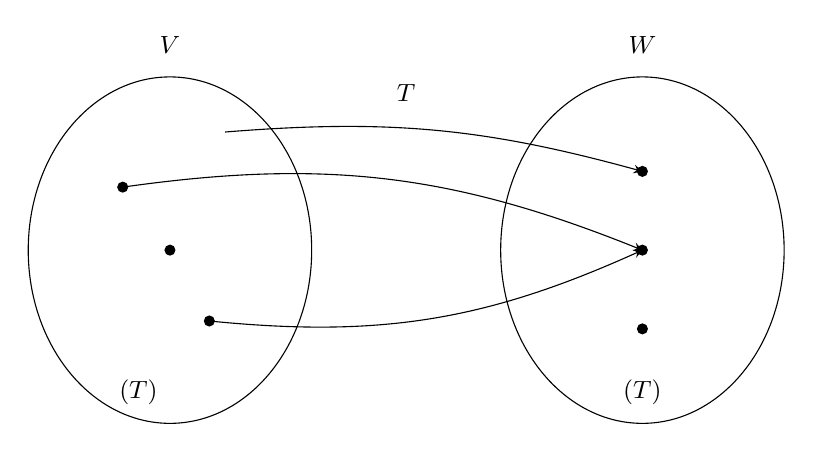
\begin{tikzpicture}[
    >=stealth,
    every node/.style={font=\small}
]
\draw (0,0) ellipse (1.8 and 2.2);
\draw (6,0) ellipse (1.8 and 2.2);

\node at (0,2.6) {\(V\)};
\node at (6,2.6) {\(W\)};

\fill (0,0) circle (2pt);
\node[left] at (0,0) {\(\zero\)};

\fill (-0.6,0.8) circle (2pt);
\fill (0.5,-0.9) circle (2pt);

\fill (6,0) circle (2pt);
\node[right] at (6,0) {\(\zero\)};

\fill (6,1) circle (2pt);
\fill (6,-1) circle (2pt);

\draw[->] (-0.6,0.8) to[bend left=15] (6,0);
\draw[->] (0.5,-0.9) to[bend right=15] (6,0);
\draw[->] (0.7,1.5) to[bend left=10] (6,1);

\node at (3,2) {\(T\)};
\node at (-0.4,-1.8) {\(\Ker(T)\)};
\node at (6,-1.8) {\(\Image(T)\)};
\end{tikzpicture}
\end{center}

The kernel contains inputs mapped to zero.

The image contains outputs actually reached.

%%%%%%%%%%%%%%%%%%%%%%%%%%%%%%%%%%%%%%%%%%%%%%%%%%%%%%%%%%%%
\subsection{Rank and Nullity}
\label{subsec:rank-nullity-intro}
%%%%%%%%%%%%%%%%%%%%%%%%%%%%%%%%%%%%%%%%%%%%%%%%%%%%%%%%%%%%

The rank of a matrix is

\[ \rank(A)=\dim(\operatorname{Col}(A)). \]

The nullity is

\[ \nullity(A)=\dim(\operatorname{Nul}(A)). \]

%%%%%%%%%%%%%%%%%%%%%%%%%%%%%%%%%%%%%%%%%%%%%%%%%%%%%%%%%%%%
\subsection{Rank--Nullity Theorem}
\label{subsec:rank-nullity}
%%%%%%%%%%%%%%%%%%%%%%%%%%%%%%%%%%%%%%%%%%%%%%%%%%%%%%%%%%%%

\begin{theorem}[Rank--Nullity Theorem]
If \(A\) has \(n\) columns, then
\[ \rank(A)+\nullity(A)=n. \]
\end{theorem}

Visually, the input dimensions split into:

\begin{center}
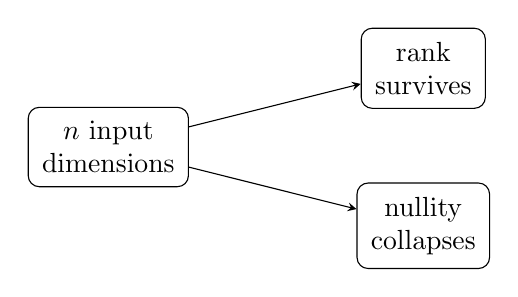
\begin{tikzpicture}[
    box/.style={draw,rounded corners,inner sep=5pt,align=center},
    >=stealth
]
\node[box] (input) at (0,0) {\(n\) input\\dimensions};
\node[box] (rank) at (4,1) {rank\\survives};
\node[box] (null) at (4,-1) {nullity\\collapses};

\draw[->] (input)--(rank);
\draw[->] (input)--(null);
\end{tikzpicture}
\end{center}

%%%%%%%%%%%%%%%%%%%%%%%%%%%%%%%%%%%%%%%%%%%%%%%%%%%%%%%%%%%%
\subsection{Linear Transformations}
\label{subsec:linear-transformations}
%%%%%%%%%%%%%%%%%%%%%%%%%%%%%%%%%%%%%%%%%%%%%%%%%%%%%%%%%%%%

\begin{definitionbox}{Linear Transformation}
A function
\[ T:V\to W \]
is linear if
\[ T(\vect{u}+\vect{v})=T(\vect{u})+T(\vect{v}) \]
and
\[ T(c\vect{v})=cT(\vect{v}). \]
\end{definitionbox}

Linear transformations preserve linear combinations.

%%%%%%%%%%%%%%%%%%%%%%%%%%%%%%%%%%%%%%%%%%%%%%%%%%%%%%%%%%%%
\subsection{Matrices as Transformations}
\label{subsec:matrices-transformations}
%%%%%%%%%%%%%%%%%%%%%%%%%%%%%%%%%%%%%%%%%%%%%%%%%%%%%%%%%%%%

Every \(m\times n\) matrix defines a transformation

\[ T:\R^n\to\R^m,\qquad T(\vect{x})=A\vect{x}. \]

A matrix can therefore be understood not merely as an array of numbers but as
a machine that transforms vectors.

%%%%%%%%%%%%%%%%%%%%%%%%%%%%%%%%%%%%%%%%%%%%%%%%%%%%%%%%%%%%
\subsection{Visualizing a Linear Transformation}
\label{subsec:visual-linear-transformation}
%%%%%%%%%%%%%%%%%%%%%%%%%%%%%%%%%%%%%%%%%%%%%%%%%%%%%%%%%%%%

Consider the transformation

\[ T(x,y)=(2x,y). \]

It stretches the plane horizontally.

\begin{center}
\begin{minipage}{0.44\textwidth}
\centering
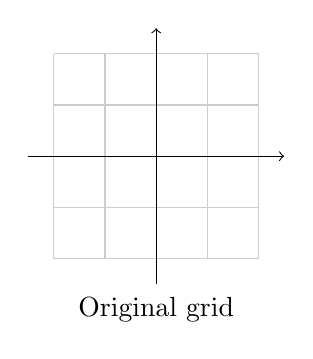
\begin{tikzpicture}[scale=0.65]
\draw[step=1cm,gray!40] (-2,-2) grid (2,2);
\draw[->] (-2.5,0)--(2.5,0);
\draw[->] (0,-2.5)--(0,2.5);
\node at (0,-3) {Original grid};
\end{tikzpicture}
\end{minipage}
\hfill
\begin{minipage}{0.44\textwidth}
\centering
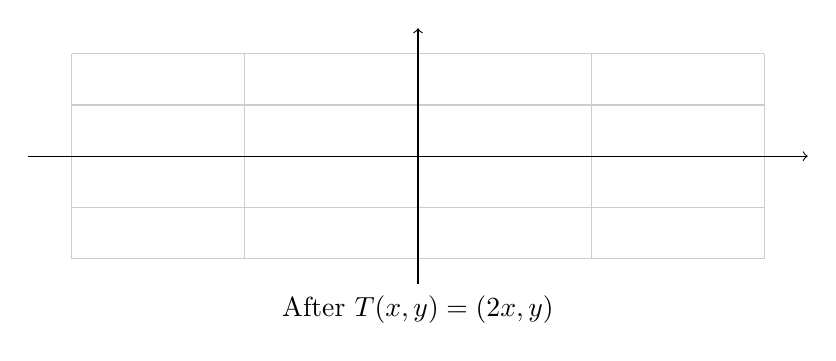
\begin{tikzpicture}[xscale=1.1,yscale=0.65]
\foreach \x in {-4,-2,0,2,4}
    \draw[gray!40] (\x,-2)--(\x,2);
\foreach \y in {-2,-1,0,1,2}
    \draw[gray!40] (-4,\y)--(4,\y);
\draw[->] (-4.5,0)--(4.5,0);
\draw[->] (0,-2.5)--(0,2.5);
\node at (0,-3) {After \(T(x,y)=(2x,y)\)};
\end{tikzpicture}
\end{minipage}
\end{center}

%%%%%%%%%%%%%%%%%%%%%%%%%%%%%%%%%%%%%%%%%%%%%%%%%%%%%%%%%%%%
\subsection{Common Geometric Linear Transformations}
\label{subsec:common-transformations}
%%%%%%%%%%%%%%%%%%%%%%%%%%%%%%%%%%%%%%%%%%%%%%%%%%%%%%%%%%%%

Matrices can represent transformations such as:

\begin{itemize}
    \item stretching;
    \item compression;
    \item reflection;
    \item rotation;
    \item shear;
    \item projection.
\end{itemize}

%%%%%%%%%%%%%%%%%%%%%%%%%%%%%%%%%%%%%%%%%%%%%%%%%%%%%%%%%%%%
\subsection{Shear Transformation}
\label{subsec:shear-transformation}
%%%%%%%%%%%%%%%%%%%%%%%%%%%%%%%%%%%%%%%%%%%%%%%%%%%%%%%%%%%%

The matrix

\[ A=\begin{bmatrix}1&1\\0&1\end{bmatrix} \]

produces a horizontal shear.

\begin{center}
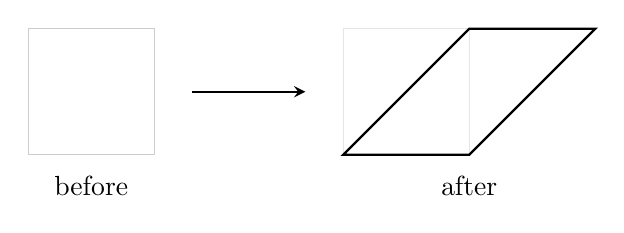
\begin{tikzpicture}[scale=0.8,>=stealth]
\draw[gray!40] (0,0) rectangle (2,2);
\node at (1,-0.5) {before};

\begin{scope}[xshift=5cm]
\draw[gray!20] (0,0) rectangle (2,2);
\draw[thick] (0,0)--(2,0)--(4,2)--(2,2)--cycle;
\node at (2,-0.5) {after};
\end{scope}

\draw[->,thick] (2.6,1)--(4.4,1);
\end{tikzpicture}
\end{center}

%%%%%%%%%%%%%%%%%%%%%%%%%%%%%%%%%%%%%%%%%%%%%%%%%%%%%%%%%%%%
\subsection{Kernel}
\label{subsec:kernel-linear-transformation}
%%%%%%%%%%%%%%%%%%%%%%%%%%%%%%%%%%%%%%%%%%%%%%%%%%%%%%%%%%%%

\begin{definitionbox}{Kernel}
The kernel of \(T:V\to W\) is
\[ \Ker(T)=\{\vect{v}\in V:T(\vect{v})=\zero\}. \]
\end{definitionbox}

%%%%%%%%%%%%%%%%%%%%%%%%%%%%%%%%%%%%%%%%%%%%%%%%%%%%%%%%%%%%
\subsection{Image}
\label{subsec:image-linear-transformation}
%%%%%%%%%%%%%%%%%%%%%%%%%%%%%%%%%%%%%%%%%%%%%%%%%%%%%%%%%%%%

\begin{definitionbox}{Image}
The image of \(T\) is
\[ \Image(T)=\{T(\vect{v}):\vect{v}\in V\}. \]
\end{definitionbox}

For

\[ T(\vect{x})=A\vect{x}, \]

\[ \Image(T)=\operatorname{Col}(A). \]

%%%%%%%%%%%%%%%%%%%%%%%%%%%%%%%%%%%%%%%%%%%%%%%%%%%%%%%%%%%%
\subsection{Injectivity and the Kernel}
\label{subsec:injectivity-kernel}
%%%%%%%%%%%%%%%%%%%%%%%%%%%%%%%%%%%%%%%%%%%%%%%%%%%%%%%%%%%%

\begin{theorem}
A linear transformation \(T\) is injective if and only if
\[ \Ker(T)=\{\zero\}. \]
\end{theorem}

\begin{proof}
Suppose \(T\) is injective. Since
\[ T(\zero)=\zero, \]
injectivity implies that no other vector maps to \(\zero\). Hence
\[ \Ker(T)=\{\zero\}. \]

Conversely, suppose
\[ \Ker(T)=\{\zero\}. \]
If
\[ T(\vect{u})=T(\vect{v}), \]
then
\[ T(\vect{u}-\vect{v})=\zero. \]
Therefore
\[ \vect{u}-\vect{v}\in\Ker(T), \]
so
\[ \vect{u}=\vect{v}. \]
Hence \(T\) is injective.
\end{proof}

%%%%%%%%%%%%%%%%%%%%%%%%%%%%%%%%%%%%%%%%%%%%%%%%%%%%%%%%%%%%
\subsection{The Invertible Matrix Theorem}
\label{subsec:invertible-matrix-theorem}
%%%%%%%%%%%%%%%%%%%%%%%%%%%%%%%%%%%%%%%%%%%%%%%%%%%%%%%%%%%%

For an \(n\times n\) matrix \(A\), the following statements are equivalent:

\begin{itemize}
    \item \(A\) is invertible;
    \item \(A\) has \(n\) pivots;
    \item \(\operatorname{RREF}(A)=I_n\);
    \item \(A\vect{x}=\zero\) has only the trivial solution;
    \item the columns are linearly independent;
    \item the columns span \(\R^n\);
    \item \(\det(A)\neq0\);
    \item \(T(\vect{x})=A\vect{x}\) is injective;
    \item \(T(\vect{x})=A\vect{x}\) is surjective.
\end{itemize}

%%%%%%%%%%%%%%%%%%%%%%%%%%%%%%%%%%%%%%%%%%%%%%%%%%%%%%%%%%%%
\subsection{Structural View of Invertibility}
\label{subsec:visual-invertibility}
%%%%%%%%%%%%%%%%%%%%%%%%%%%%%%%%%%%%%%%%%%%%%%%%%%%%%%%%%%%%

\begin{center}
\begin{tikzpicture}[
    node distance=11mm,
    box/.style={draw,rounded corners,align=center,inner sep=4pt,font=\small},
    >=stealth
]
\node[box] (inv) {Invertible};
\node[box,below left=of inv] (det) {\(\det(A)\neq0\)};
\node[box,below=of inv] (pivot) {\(n\) pivots};
\node[box,below right=of inv] (basis) {columns form\\a basis};
\node[box,below=22mm of inv] (bij) {linear transformation\\is bijective};

\draw[<->] (inv)--(det);
\draw[<->] (inv)--(pivot);
\draw[<->] (inv)--(basis);
\draw[<->] (inv)--(bij);
\end{tikzpicture}
\end{center}

These are different descriptions of the same underlying structure.

%%%%%%%%%%%%%%%%%%%%%%%%%%%%%%%%%%%%%%%%%%%%%%%%%%%%%%%%%%%%
\subsection{Eigenvalues and Eigenvectors}
\label{subsec:eigenvalues-eigenvectors}
%%%%%%%%%%%%%%%%%%%%%%%%%%%%%%%%%%%%%%%%%%%%%%%%%%%%%%%%%%%%

\begin{definitionbox}{Eigenvalue and Eigenvector}
For a square matrix \(A\), a nonzero vector \(\vect{v}\) is an eigenvector if
\[ A\vect{v}=\lambda\vect{v} \]
for some scalar \(\lambda\). The scalar \(\lambda\) is the corresponding
eigenvalue.
\end{definitionbox}

The symbol

\[ \lambda \]

is lowercase Greek \emph{lambda}, pronounced ``LAM-duh.''

%%%%%%%%%%%%%%%%%%%%%%%%%%%%%%%%%%%%%%%%%%%%%%%%%%%%%%%%%%%%
\subsection{Geometric Meaning of an Eigenvector}
\label{subsec:geometric-eigenvectors}
%%%%%%%%%%%%%%%%%%%%%%%%%%%%%%%%%%%%%%%%%%%%%%%%%%%%%%%%%%%%

Most vectors change direction under a transformation.

An eigenvector remains on the same line through the origin.

\begin{center}
\begin{tikzpicture}[scale=0.9,>=stealth]
\draw[->] (-0.5,0)--(5,0);
\draw[->] (0,-0.5)--(0,3.5);

\draw[dashed] (-0.3,-0.15)--(4.8,2.4);

\draw[->,very thick] (0,0)--(2,1)
node[midway,above]{\(\vect{v}\)};

\draw[->,very thick] (0,0)--(4,2)
node[right]{\(A\vect{v}=\lambda\vect{v}\)};
\end{tikzpicture}
\end{center}

The transformation may stretch, shrink, reverse, or collapse the vector, but
does not change its line of direction.

%%%%%%%%%%%%%%%%%%%%%%%%%%%%%%%%%%%%%%%%%%%%%%%%%%%%%%%%%%%%
\subsection{Finding Eigenvalues}
\label{subsec:finding-eigenvalues}
%%%%%%%%%%%%%%%%%%%%%%%%%%%%%%%%%%%%%%%%%%%%%%%%%%%%%%%%%%%%

Starting from

\[ A\vect{v}=\lambda\vect{v}, \]

we obtain

\[ (A-\lambda I)\vect{v}=\zero. \]

A nonzero solution exists only if

\[ A-\lambda I \]

is noninvertible.

Therefore,

\[ \det(A-\lambda I)=0. \]

This is the characteristic equation.

%%%%%%%%%%%%%%%%%%%%%%%%%%%%%%%%%%%%%%%%%%%%%%%%%%%%%%%%%%%%
\subsection{Characteristic Polynomial}
\label{subsec:characteristic-polynomial}
%%%%%%%%%%%%%%%%%%%%%%%%%%%%%%%%%%%%%%%%%%%%%%%%%%%%%%%%%%%%

The polynomial

\[ p_A(\lambda)=\det(A-\lambda I) \]

is the characteristic polynomial.

Its roots are the eigenvalues.

%%%%%%%%%%%%%%%%%%%%%%%%%%%%%%%%%%%%%%%%%%%%%%%%%%%%%%%%%%%%
\subsection{Worked Example: Eigenvalues and Eigenvectors}
\label{subsec:worked-eigenvalues}
%%%%%%%%%%%%%%%%%%%%%%%%%%%%%%%%%%%%%%%%%%%%%%%%%%%%%%%%%%%%

\begin{workedexamplebox}{Find Eigenvalues and Eigenvectors}

Let

\[ A=\begin{bmatrix}2&1\\0&3\end{bmatrix}. \]

\begin{tabularx}{\textwidth}{@{}>{\raggedright\arraybackslash}p{0.42\textwidth}X@{}}
Form \(A-\lambda I\). &
\(\begin{bmatrix}2-\lambda&1\\0&3-\lambda\end{bmatrix}\)\\[2mm]
Compute determinant. &
\((2-\lambda)(3-\lambda)\)\\
Solve. &
\(\lambda=2,3\)\\
For \(\lambda=2\). &
\(\vect{v}=t\begin{bmatrix}1\\0\end{bmatrix}\)\\[2mm]
For \(\lambda=3\). &
\(\vect{v}=t\begin{bmatrix}1\\1\end{bmatrix}\)
\end{tabularx}

\begin{answerbox}
\[ \lambda_1=2,\quad \vect{v}_1=\begin{bmatrix}1\\0\end{bmatrix},
\qquad
\lambda_2=3,\quad \vect{v}_2=\begin{bmatrix}1\\1\end{bmatrix} \]
\end{answerbox}
\end{workedexamplebox}

%%%%%%%%%%%%%%%%%%%%%%%%%%%%%%%%%%%%%%%%%%%%%%%%%%%%%%%%%%%%
\subsection{Eigenspaces}
\label{subsec:eigenspaces}
%%%%%%%%%%%%%%%%%%%%%%%%%%%%%%%%%%%%%%%%%%%%%%%%%%%%%%%%%%%%

For eigenvalue \(\lambda\),

\[ E_\lambda=\Ker(A-\lambda I). \]

The eigenspace contains every eigenvector associated with \(\lambda\) together
with the zero vector.

%%%%%%%%%%%%%%%%%%%%%%%%%%%%%%%%%%%%%%%%%%%%%%%%%%%%%%%%%%%%
\subsection{Diagonalization}
\label{subsec:diagonalization}
%%%%%%%%%%%%%%%%%%%%%%%%%%%%%%%%%%%%%%%%%%%%%%%%%%%%%%%%%%%%

\begin{definitionbox}{Diagonalizable Matrix}
A matrix \(A\) is diagonalizable if
\[ A=PDP^{-1}, \]
where \(P\) is invertible and \(D\) is diagonal.
\end{definitionbox}

The columns of \(P\) are linearly independent eigenvectors.

The corresponding eigenvalues appear on the diagonal of \(D\).

%%%%%%%%%%%%%%%%%%%%%%%%%%%%%%%%%%%%%%%%%%%%%%%%%%%%%%%%%%%%
\subsection{Diagonalization as a Change of Coordinates}
\label{subsec:diagonalization-visual}
%%%%%%%%%%%%%%%%%%%%%%%%%%%%%%%%%%%%%%%%%%%%%%%%%%%%%%%%%%%%

Conceptually,

\begin{center}
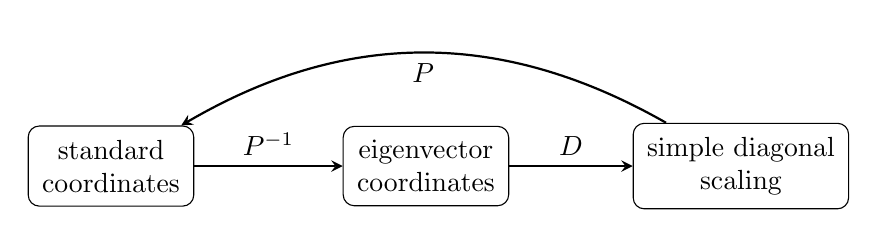
\begin{tikzpicture}[
    box/.style={draw,rounded corners,align=center,inner sep=5pt},
    >=stealth
]
\node[box] (std) at (0,0) {standard\\coordinates};
\node[box] (eig) at (4,0) {eigenvector\\coordinates};
\node[box] (scale) at (8,0) {simple diagonal\\scaling};

\draw[->,thick] (std)--node[above]{\(P^{-1}\)}(eig);
\draw[->,thick] (eig)--node[above]{\(D\)}(scale);
\draw[->,bend right=30,thick] (scale) to node[below]{\(P\)} (std);
\end{tikzpicture}
\end{center}

Diagonalization finds coordinates in which the transformation becomes simple
scaling along eigenvector directions.

%%%%%%%%%%%%%%%%%%%%%%%%%%%%%%%%%%%%%%%%%%%%%%%%%%%%%%%%%%%%
\subsection{Dot Product}
\label{subsec:dot-product}
%%%%%%%%%%%%%%%%%%%%%%%%%%%%%%%%%%%%%%%%%%%%%%%%%%%%%%%%%%%%

For

\[ \vect{u}=\begin{bmatrix}u_1\\\vdots\\u_n\end{bmatrix},
\qquad
\vect{v}=\begin{bmatrix}v_1\\\vdots\\v_n\end{bmatrix}, \]

the dot product is

\[ \vect{u}\cdot\vect{v}
=u_1v_1+\cdots+u_nv_n. \]

Equivalently,

\[ \vect{u}\cdot\vect{v}=\vect{u}^{\mathsf T}\vect{v}. \]

%%%%%%%%%%%%%%%%%%%%%%%%%%%%%%%%%%%%%%%%%%%%%%%%%%%%%%%%%%%%
\subsection{Norm}
\label{subsec:vector-norm}
%%%%%%%%%%%%%%%%%%%%%%%%%%%%%%%%%%%%%%%%%%%%%%%%%%%%%%%%%%%%

The Euclidean norm is

\[ \norm{\vect{v}}=\sqrt{\vect{v}\cdot\vect{v}}. \]

It is read ``the norm of \(\vect{v}\).''

For

\[ \vect{v}=\begin{bmatrix}3\\4\end{bmatrix}, \]

\[ \norm{\vect{v}}=5. \]

%%%%%%%%%%%%%%%%%%%%%%%%%%%%%%%%%%%%%%%%%%%%%%%%%%%%%%%%%%%%
\subsection{Visualizing Vector Length}
\label{subsec:visual-vector-length}
%%%%%%%%%%%%%%%%%%%%%%%%%%%%%%%%%%%%%%%%%%%%%%%%%%%%%%%%%%%%

\begin{center}
\begin{tikzpicture}[scale=0.9,>=stealth]
\draw[->] (-0.5,0)--(5,0);
\draw[->] (0,-0.5)--(0,4);

\draw[->,very thick] (0,0)--(4,3)
node[midway,above left]{\(\norm{\vect{v}}\)};

\draw[dashed] (4,0)--(4,3);
\draw[dashed] (0,3)--(4,3);

\node[below] at (2,0) {\(v_1\)};
\node[right] at (4,1.5) {\(v_2\)};
\end{tikzpicture}
\end{center}

By the Pythagorean theorem,

\[ \norm{\vect{v}}=\sqrt{v_1^2+v_2^2}. \]

%%%%%%%%%%%%%%%%%%%%%%%%%%%%%%%%%%%%%%%%%%%%%%%%%%%%%%%%%%%%
\subsection{Orthogonality}
\label{subsec:orthogonality}
%%%%%%%%%%%%%%%%%%%%%%%%%%%%%%%%%%%%%%%%%%%%%%%%%%%%%%%%%%%%

\begin{definitionbox}{Orthogonal Vectors}
Vectors \(\vect{u}\) and \(\vect{v}\) are orthogonal if
\[ \vect{u}\cdot\vect{v}=0. \]
\end{definitionbox}

Geometrically, orthogonal vectors meet at a right angle.

\begin{center}
\begin{tikzpicture}[scale=0.9,>=stealth]
\draw[->] (-0.5,0)--(5,0);
\draw[->] (0,-0.5)--(0,4);

\draw[->,very thick] (0,0)--(4,1)
node[right]{\(\vect{u}\)};

\draw[->,very thick] (0,0)--(-0.8,3.2)
node[above]{\(\vect{v}\)};

\draw (0.42,0.1)--(0.32,0.5)--(-0.08,0.4);
\end{tikzpicture}
\end{center}

%%%%%%%%%%%%%%%%%%%%%%%%%%%%%%%%%%%%%%%%%%%%%%%%%%%%%%%%%%%%
\subsection{Angle Between Vectors}
\label{subsec:angle-between-vectors}
%%%%%%%%%%%%%%%%%%%%%%%%%%%%%%%%%%%%%%%%%%%%%%%%%%%%%%%%%%%%

For nonzero vectors,

\[ \vect{u}\cdot\vect{v}
=\norm{\vect{u}}\norm{\vect{v}}\cos\theta. \]

The symbol

\[ \theta \]

is lowercase Greek \emph{theta}, pronounced ``THAY-tuh'' or ``THEE-tuh.''

Thus,

\[ \cos\theta=
\frac{\vect{u}\cdot\vect{v}}
{\norm{\vect{u}}\norm{\vect{v}}}. \]

%%%%%%%%%%%%%%%%%%%%%%%%%%%%%%%%%%%%%%%%%%%%%%%%%%%%%%%%%%%%
\subsection{Visualizing the Angle}
\label{subsec:visual-vector-angle}
%%%%%%%%%%%%%%%%%%%%%%%%%%%%%%%%%%%%%%%%%%%%%%%%%%%%%%%%%%%%

\begin{center}
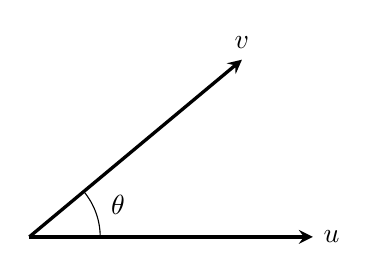
\begin{tikzpicture}[scale=0.9,>=stealth]
\draw[->,very thick] (0,0)--(4,0)
node[right]{\(\vect{u}\)};

\draw[->,very thick] (0,0)--(3,2.5)
node[above]{\(\vect{v}\)};

\draw (1,0) arc[start angle=0,end angle=40,radius=1];
\node at (1.25,0.45) {\(\theta\)};
\end{tikzpicture}
\end{center}

%%%%%%%%%%%%%%%%%%%%%%%%%%%%%%%%%%%%%%%%%%%%%%%%%%%%%%%%%%%%
\subsection{Cauchy--Schwarz Inequality}
\label{subsec:cauchy-schwarz-linear-algebra}
%%%%%%%%%%%%%%%%%%%%%%%%%%%%%%%%%%%%%%%%%%%%%%%%%%%%%%%%%%%%

\begin{theorem}[Cauchy--Schwarz Inequality]
For vectors \(\vect{u},\vect{v}\in\R^n\),
\[ |\vect{u}\cdot\vect{v}|
\leq\norm{\vect{u}}\norm{\vect{v}}. \]
\end{theorem}

This inequality is fundamental throughout linear algebra and analysis.

%%%%%%%%%%%%%%%%%%%%%%%%%%%%%%%%%%%%%%%%%%%%%%%%%%%%%%%%%%%%
\subsection{Orthogonal Projection}
\label{subsec:orthogonal-projection}
%%%%%%%%%%%%%%%%%%%%%%%%%%%%%%%%%%%%%%%%%%%%%%%%%%%%%%%%%%%%

The projection of \(\vect{v}\) onto a nonzero vector \(\vect{u}\) is

\[ \operatorname{proj}_{\vect{u}}(\vect{v})
=
\frac{\vect{v}\cdot\vect{u}}
{\vect{u}\cdot\vect{u}}\vect{u}. \]

%%%%%%%%%%%%%%%%%%%%%%%%%%%%%%%%%%%%%%%%%%%%%%%%%%%%%%%%%%%%
\subsection{Visualizing Projection}
\label{subsec:visual-projection}
%%%%%%%%%%%%%%%%%%%%%%%%%%%%%%%%%%%%%%%%%%%%%%%%%%%%%%%%%%%%

\begin{center}
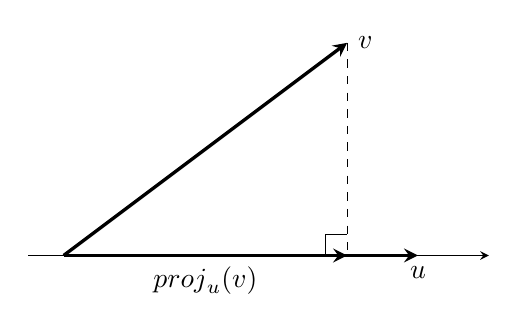
\begin{tikzpicture}[scale=0.9,>=stealth]
\draw[->] (-0.5,0)--(6,0);

\draw[->,very thick] (0,0)--(4,3)
node[right]{\(\vect{v}\)};

\draw[->,very thick] (0,0)--(5,0)
node[below]{\(\vect{u}\)};

\draw[dashed] (4,3)--(4,0);

\draw[->,very thick] (0,0)--(4,0)
node[midway,below]{\(\operatorname{proj}_{\vect{u}}(\vect{v})\)};

\draw (3.7,0)--(3.7,0.3)--(4,0.3);
\end{tikzpicture}
\end{center}

The projection is the component of \(\vect{v}\) lying in the direction of
\(\vect{u}\).

%%%%%%%%%%%%%%%%%%%%%%%%%%%%%%%%%%%%%%%%%%%%%%%%%%%%%%%%%%%%
\subsection{Worked Example: Projection}
\label{subsec:worked-vector-projection}
%%%%%%%%%%%%%%%%%%%%%%%%%%%%%%%%%%%%%%%%%%%%%%%%%%%%%%%%%%%%

\begin{workedexamplebox}{Project One Vector onto Another}

Let

\[ \vect{v}=\begin{bmatrix}3\\4\end{bmatrix},\qquad
\vect{u}=\begin{bmatrix}1\\0\end{bmatrix}. \]

\begin{tabularx}{\textwidth}{@{}>{\raggedright\arraybackslash}p{0.42\textwidth}X@{}}
Compute dot product. & \(\vect{v}\cdot\vect{u}=3\)\\
Compute \(\vect{u}\cdot\vect{u}\). & \(1\)\\
Apply projection formula. & \(3\vect{u}\)
\end{tabularx}

\begin{answerbox}
\[ \operatorname{proj}_{\vect{u}}(\vect{v})
=\begin{bmatrix}3\\0\end{bmatrix} \]
\end{answerbox}
\end{workedexamplebox}

%%%%%%%%%%%%%%%%%%%%%%%%%%%%%%%%%%%%%%%%%%%%%%%%%%%%%%%%%%%%
\subsection{Orthogonal Complements}
\label{subsec:orthogonal-complements}
%%%%%%%%%%%%%%%%%%%%%%%%%%%%%%%%%%%%%%%%%%%%%%%%%%%%%%%%%%%%

For a subspace \(W\subseteq\R^n\),

\[ W^\perp=
\{\vect{v}\in\R^n:\vect{v}\cdot\vect{w}=0
\text{ for all }\vect{w}\in W\}. \]

The symbol

\[ \perp \]

is called the perpendicular symbol and is read ``perpendicular to'' or
``orthogonal to.''

%%%%%%%%%%%%%%%%%%%%%%%%%%%%%%%%%%%%%%%%%%%%%%%%%%%%%%%%%%%%
\subsection{Gram--Schmidt Process}
\label{subsec:gram-schmidt}
%%%%%%%%%%%%%%%%%%%%%%%%%%%%%%%%%%%%%%%%%%%%%%%%%%%%%%%%%%%%

The Gram--Schmidt process converts an independent set into an orthogonal set
with the same span.

Starting with

\[ \vect{v}_1,\vect{v}_2, \]

set

\[ \vect{u}_1=\vect{v}_1. \]

Then

\[ \vect{u}_2
=
\vect{v}_2-\operatorname{proj}_{\vect{u}_1}(\vect{v}_2). \]

%%%%%%%%%%%%%%%%%%%%%%%%%%%%%%%%%%%%%%%%%%%%%%%%%%%%%%%%%%%%
\subsection{Visualizing Gram--Schmidt}
\label{subsec:visual-gram-schmidt}
%%%%%%%%%%%%%%%%%%%%%%%%%%%%%%%%%%%%%%%%%%%%%%%%%%%%%%%%%%%%

\begin{center}
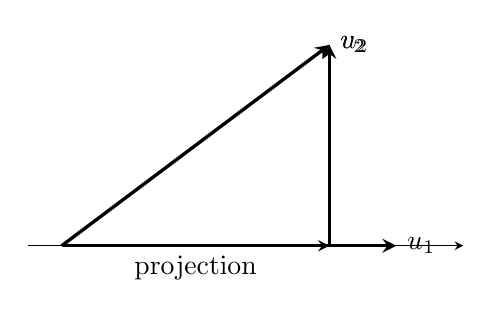
\begin{tikzpicture}[scale=0.85,>=stealth]
\draw[->] (-0.5,0)--(6,0);

\draw[->,very thick] (0,0)--(5,0)
node[right]{\(\vect{u}_1\)};

\draw[->,very thick] (0,0)--(4,3)
node[right]{\(\vect{v}_2\)};

\draw[dashed] (4,3)--(4,0);

\draw[->,thick] (0,0)--(4,0)
node[midway,below]{projection};

\draw[->,very thick] (4,0)--(4,3)
node[right]{\(\vect{u}_2\)};
\end{tikzpicture}
\end{center}

The projection component is removed, leaving an orthogonal direction.

%%%%%%%%%%%%%%%%%%%%%%%%%%%%%%%%%%%%%%%%%%%%%%%%%%%%%%%%%%%%
\subsection{Least-Squares Approximation}
\label{subsec:least-squares}
%%%%%%%%%%%%%%%%%%%%%%%%%%%%%%%%%%%%%%%%%%%%%%%%%%%%%%%%%%%%

A system

\[ A\vect{x}=\vect{b} \]

may have no exact solution.

Instead, least squares seeks

\[ \widehat{\vect{x}} \]

such that

\[ A\widehat{\vect{x}} \]

is as close as possible to \(\vect{b}\).

The notation

\[ \widehat{\vect{x}} \]

is read ``\(x\) hat.''

%%%%%%%%%%%%%%%%%%%%%%%%%%%%%%%%%%%%%%%%%%%%%%%%%%%%%%%%%%%%
\subsection{Geometric Meaning of Least Squares}
\label{subsec:least-squares-geometry}
%%%%%%%%%%%%%%%%%%%%%%%%%%%%%%%%%%%%%%%%%%%%%%%%%%%%%%%%%%%%

The vector

\[ A\widehat{\vect{x}} \]

is the orthogonal projection of \(\vect{b}\) onto the column space of \(A\).

\begin{center}
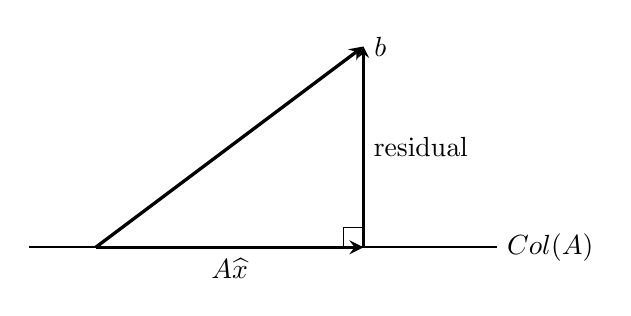
\begin{tikzpicture}[scale=0.85,>=stealth]
\draw[thick] (-1,0)--(6,0);
\node[right] at (6,0) {\(\operatorname{Col}(A)\)};

\draw[->,very thick] (0,0)--(4,3)
node[right]{\(\vect{b}\)};

\draw[->,very thick] (0,0)--(4,0)
node[midway,below]{\(A\widehat{\vect{x}}\)};

\draw[dashed] (4,3)--(4,0);
\draw[->,thick] (4,0)--(4,3)
node[midway,right]{residual};

\draw (3.7,0)--(3.7,0.3)--(4,0.3);
\end{tikzpicture}
\end{center}

The residual

\[ \vect{b}-A\widehat{\vect{x}} \]

is orthogonal to the column space.

%%%%%%%%%%%%%%%%%%%%%%%%%%%%%%%%%%%%%%%%%%%%%%%%%%%%%%%%%%%%
\subsection{Normal Equations}
\label{subsec:normal-equations}
%%%%%%%%%%%%%%%%%%%%%%%%%%%%%%%%%%%%%%%%%%%%%%%%%%%%%%%%%%%%

Orthogonality of the residual implies

\[ A^{\mathsf T}
(\vect{b}-A\widehat{\vect{x}})=\zero. \]

Therefore,

\[ A^{\mathsf T}A\widehat{\vect{x}}
=
A^{\mathsf T}\vect{b}. \]

These are the \emph{normal equations}.

If \(A^{\mathsf T}A\) is invertible,

\[ \widehat{\vect{x}}
=
(A^{\mathsf T}A)^{-1}A^{\mathsf T}\vect{b}. \]

Least squares forms the mathematical foundation of ordinary linear regression.

%%%%%%%%%%%%%%%%%%%%%%%%%%%%%%%%%%%%%%%%%%%%%%%%%%%%%%%%%%%%
\subsection{Applications of Linear Algebra}
\label{subsec:linear-algebra-applications}
%%%%%%%%%%%%%%%%%%%%%%%%%%%%%%%%%%%%%%%%%%%%%%%%%%%%%%%%%%%%

Linear algebra supports a wide variety of mathematical models.

\begin{applicationbox}
\textbf{Differential equations:}
systems such as
\[ \dv{\vect{x}}{t}=A\vect{x} \]
can be studied using eigenvalues and eigenvectors.
\end{applicationbox}

\begin{applicationbox}
\textbf{Statistics:}
least squares and regression are naturally expressed using matrices and
projections.
\end{applicationbox}

\begin{applicationbox}
\textbf{Computer graphics:}
rotations, reflections, scaling, and perspective calculations use matrix
transformations.
\end{applicationbox}

\begin{applicationbox}
\textbf{Data science:}
datasets are naturally represented as matrices whose rows represent
observations and columns represent variables.
\end{applicationbox}

%%%%%%%%%%%%%%%%%%%%%%%%%%%%%%%%%%%%%%%%%%%%%%%%%%%%%%%%%%%%
\subsection{Common Linear Algebra Errors}
\label{subsec:common-linear-algebra-errors}
%%%%%%%%%%%%%%%%%%%%%%%%%%%%%%%%%%%%%%%%%%%%%%%%%%%%%%%%%%%%

\subsubsection{Multiplying Matrices Entrywise}

Ordinary matrix multiplication is row-by-column multiplication.

%%%%%%%%%%%%%%%%%%%%%%%%%%%%%%%%%%%%%%%%%%%%%%%%%%%%%%%%%%%%
\subsubsection{Assuming Multiplication Commutes}
\label{subsec:error-matrix-commutative}
%%%%%%%%%%%%%%%%%%%%%%%%%%%%%%%%%%%%%%%%%%%%%%%%%%%%%%%%%%%%

In general,

\[ AB\neq BA. \]

%%%%%%%%%%%%%%%%%%%%%%%%%%%%%%%%%%%%%%%%%%%%%%%%%%%%%%%%%%%%
\subsubsection{Ignoring Dimensions}
\label{subsec:error-matrix-dimensions}
%%%%%%%%%%%%%%%%%%%%%%%%%%%%%%%%%%%%%%%%%%%%%%%%%%%%%%%%%%%%

For

\[ A_{m\times n}B_{r\times p}, \]

the product exists only if

\[ n=r. \]

%%%%%%%%%%%%%%%%%%%%%%%%%%%%%%%%%%%%%%%%%%%%%%%%%%%%%%%%%%%%
\subsubsection{Confusing Span and Independence}
\label{subsec:error-span-independence}
%%%%%%%%%%%%%%%%%%%%%%%%%%%%%%%%%%%%%%%%%%%%%%%%%%%%%%%%%%%%

A spanning set may contain redundant vectors.

An independent set may fail to span the whole space.

A basis requires both properties.

%%%%%%%%%%%%%%%%%%%%%%%%%%%%%%%%%%%%%%%%%%%%%%%%%%%%%%%%%%%%
\subsubsection{Assuming Every Matrix Is Invertible}
\label{subsec:error-all-matrices-invertible}
%%%%%%%%%%%%%%%%%%%%%%%%%%%%%%%%%%%%%%%%%%%%%%%%%%%%%%%%%%%%

Only square matrices can have ordinary two-sided inverses, and even square
matrices may fail to be invertible.

%%%%%%%%%%%%%%%%%%%%%%%%%%%%%%%%%%%%%%%%%%%%%%%%%%%%%%%%%%%%
\subsubsection{Treating Row-Equivalent Matrices as Equal}
\label{subsec:error-row-equivalent-equal}
%%%%%%%%%%%%%%%%%%%%%%%%%%%%%%%%%%%%%%%%%%%%%%%%%%%%%%%%%%%%

Row operations change the matrix.

If \(A\) row reduces to \(B\), then \(A\) and \(B\) are row equivalent, not
necessarily equal.

%%%%%%%%%%%%%%%%%%%%%%%%%%%%%%%%%%%%%%%%%%%%%%%%%%%%%%%%%%%%
\subsubsection{Using the Zero Vector as an Eigenvector}
\label{subsec:error-zero-eigenvector}
%%%%%%%%%%%%%%%%%%%%%%%%%%%%%%%%%%%%%%%%%%%%%%%%%%%%%%%%%%%%

An eigenvector must be nonzero.

%%%%%%%%%%%%%%%%%%%%%%%%%%%%%%%%%%%%%%%%%%%%%%%%%%%%%%%%%%%%
\subsubsection{Assuming Every Matrix Is Diagonalizable}
\label{subsec:error-diagonalizable}
%%%%%%%%%%%%%%%%%%%%%%%%%%%%%%%%%%%%%%%%%%%%%%%%%%%%%%%%%%%%

A matrix must have enough linearly independent eigenvectors to be
diagonalizable.

%%%%%%%%%%%%%%%%%%%%%%%%%%%%%%%%%%%%%%%%%%%%%%%%%%%%%%%%%%%%
\subsection{Exercises}
\label{subsec:linear-algebra-exercises}
%%%%%%%%%%%%%%%%%%%%%%%%%%%%%%%%%%%%%%%%%%%%%%%%%%%%%%%%%%%%

\begin{exercise}[1]
Determine whether
\[ 3x_1-2x_2+7x_3=4 \]
is linear.
\end{exercise}

\begin{exercise}[1]
Determine whether
\[ x_1x_2+x_3=5 \]
is linear.
\end{exercise}

\begin{exercise}[1]
Solve
\[ \begin{cases}
x+y=8,\\
x-y=2.
\end{cases} \]
Then sketch the two lines and identify the intersection.
\end{exercise}

\begin{exercise}[1]
Write the augmented matrix for
\[ \begin{cases}
2x-y+3z=4,\\
x+5y-z=7.
\end{cases} \]
\end{exercise}

\begin{exercise}[1]
Perform
\[ R_2\leftarrow R_2-3R_1 \]
on
\[ \begin{bmatrix}1&2\\5&7\end{bmatrix}. \]
\end{exercise}

\begin{exercise}[2]
Row reduce
\[ \left[\begin{array}{cc|c}
1&2&5\\
3&-1&4
\end{array}\right]. \]
\end{exercise}

\begin{exercise}[2]
Solve using Gaussian elimination:
\[ \begin{cases}
x+y+z=4,\\
2x-y+3z=9,\\
3x+2y-z=2.
\end{cases} \]
\end{exercise}

\begin{exercise}[2]
Determine whether the matrix
\[ \left[\begin{array}{ccc|c}
1&0&2&3\\
0&1&-4&5\\
0&0&0&1
\end{array}\right] \]
represents a consistent system.
\end{exercise}

\begin{exercise}[2]
Write the solution set represented by
\[ \left[\begin{array}{ccc|c}
1&0&3&2\\
0&1&-2&4
\end{array}\right] \]
in parametric vector form.
\end{exercise}

\begin{exercise}[1]
Compute
\[ \begin{bmatrix}1&3\\2&4\end{bmatrix}
+\begin{bmatrix}5&-1\\0&2\end{bmatrix}. \]
\end{exercise}

\begin{exercise}[1]
Compute
\[ -3\begin{bmatrix}2&1\\-4&5\end{bmatrix}. \]
\end{exercise}

\begin{exercise}[2]
Compute
\[ \begin{bmatrix}1&2&3\\0&-1&4\end{bmatrix}
\begin{bmatrix}2&1\\3&0\\-1&5\end{bmatrix}. \]
\end{exercise}

\begin{exercise}[2]
Find \(AB\) and \(BA\) for
\[ A=\begin{bmatrix}1&2\\0&1\end{bmatrix},\qquad
B=\begin{bmatrix}2&0\\3&1\end{bmatrix}. \]
Compare.
\end{exercise}

\begin{exercise}[1]
Compute
\[ \det\begin{bmatrix}4&2\\3&5\end{bmatrix}. \]
\end{exercise}

\begin{exercise}[2]
For
\[ A=\begin{bmatrix}2&0\\0&3\end{bmatrix}, \]
describe geometrically how \(A\) transforms the unit square and compare its
area before and after transformation.
\end{exercise}

\begin{exercise}[2]
Determine whether
\[ A=\begin{bmatrix}2&4\\1&2\end{bmatrix} \]
is invertible.
\end{exercise}

\begin{exercise}[1]
Draw
\[ \vect{u}=\begin{bmatrix}3\\1\end{bmatrix},
\qquad
\vect{v}=\begin{bmatrix}1\\2\end{bmatrix} \]
and use the tip-to-tail rule to sketch
\[ \vect{u}+\vect{v}. \]
\end{exercise}

\begin{exercise}[1]
Sketch
\[ 2\vect{v},\qquad -\vect{v} \]
for
\[ \vect{v}=\begin{bmatrix}2\\1\end{bmatrix}. \]
\end{exercise}

\begin{exercise}[2]
Determine whether
\[ \begin{bmatrix}1\\2\end{bmatrix},
\qquad
\begin{bmatrix}2\\4\end{bmatrix} \]
are linearly independent. Explain geometrically.
\end{exercise}

\begin{exercise}[2]
Determine whether
\[ \begin{bmatrix}1\\0\\1\end{bmatrix},
\begin{bmatrix}0\\1\\1\end{bmatrix},
\begin{bmatrix}1\\1\\2\end{bmatrix} \]
are linearly independent.
\end{exercise}

\begin{exercise}[2]
Determine whether
\[ W=\left\{
\begin{bmatrix}x\\y\end{bmatrix}\in\R^2:x+y=1
\right\} \]
is a subspace. Give a geometric explanation.
\end{exercise}

\begin{exercise}[2]
Find a basis for
\[ \Span\left\{
\begin{bmatrix}1\\0\\1\end{bmatrix},
\begin{bmatrix}2\\0\\2\end{bmatrix},
\begin{bmatrix}0\\1\\1\end{bmatrix}
\right\}. \]
\end{exercise}

\begin{exercise}[2]
Find the rank and nullity of
\[ A=\begin{bmatrix}1&2&3\\0&1&4\\0&0&0\end{bmatrix}. \]
\end{exercise}

\begin{exercise}[2]
Find a basis for
\[ \operatorname{Nul}(A) \]
where
\[ A=\begin{bmatrix}1&2&-1\\2&4&-2\end{bmatrix}. \]
\end{exercise}

\begin{exercise}[2]
Determine whether
\[ T(x,y)=(2x-y,x+3y) \]
defines a linear transformation.
\end{exercise}

\begin{exercise}[2]
Find the standard matrix for
\[ T(x,y)=(x+2y,3x-y). \]
\end{exercise}

\begin{exercise}[2]
Sketch how
\[ T(x,y)=(3x,y) \]
transforms the unit square.
\end{exercise}

\begin{exercise}[2]
Sketch the effect of
\[ A=\begin{bmatrix}-1&0\\0&1\end{bmatrix} \]
on several vectors. Identify the geometric transformation.
\end{exercise}

\begin{exercise}[2]
Find the kernel of
\[ T(x,y)=(x+y,2x+2y). \]
Sketch the kernel in \(\R^2\).
\end{exercise}

\begin{exercise}[2]
Find the eigenvalues of
\[ A=\begin{bmatrix}4&1\\0&2\end{bmatrix}. \]
\end{exercise}

\begin{exercise}[2]
Find an eigenvector corresponding to each eigenvalue of
\[ A=\begin{bmatrix}3&0\\0&-2\end{bmatrix}. \]
Sketch the eigenvector directions.
\end{exercise}

\begin{exercise}[3]
Determine whether
\[ A=\begin{bmatrix}1&1\\0&1\end{bmatrix} \]
is diagonalizable.
\end{exercise}

\begin{exercise}[1]
Compute
\[ \begin{bmatrix}2\\-1\\3\end{bmatrix}
\cdot
\begin{bmatrix}4\\2\\0\end{bmatrix}. \]
\end{exercise}

\begin{exercise}[1]
Find
\[ \norm{\begin{bmatrix}2\\-3\\6\end{bmatrix}}. \]
\end{exercise}

\begin{exercise}[2]
Determine whether
\[ \begin{bmatrix}1\\2\\-1\end{bmatrix}
\quad\text{and}\quad
\begin{bmatrix}3\\-1\\1\end{bmatrix} \]
are orthogonal.
\end{exercise}

\begin{exercise}[2]
Normalize
\[ \begin{bmatrix}3\\4\end{bmatrix}. \]
\end{exercise}

\begin{exercise}[2]
Find the projection of
\[ \begin{bmatrix}4\\3\end{bmatrix} \]
onto
\[ \begin{bmatrix}1\\1\end{bmatrix}. \]
Sketch the projection.
\end{exercise}

\begin{exercise}[3]
Apply the Gram--Schmidt process to
\[ \vect{v}_1=\begin{bmatrix}1\\1\\0\end{bmatrix},
\qquad
\vect{v}_2=\begin{bmatrix}1\\0\\1\end{bmatrix}. \]
\end{exercise}

\begin{exercise}[3]
Explain geometrically why the least-squares residual must be orthogonal to
\(\operatorname{Col}(A)\).
\end{exercise}

\begin{exercise}[3]
Prove that eigenvectors corresponding to distinct eigenvalues are linearly
independent.
\end{exercise}

\begin{exercise}[3]
Prove that
\[ \operatorname{Nul}(A) \]
is a subspace.
\end{exercise}

\begin{exercise}[3]
Prove that the columns of an invertible square matrix are linearly independent.
\end{exercise}

%%%%%%%%%%%%%%%%%%%%%%%%%%%%%%%%%%%%%%%%%%%%%%%%%%%%%%%%%%%%
\subsection{Section Connections}
\label{subsec:linear-algebra-connections}
%%%%%%%%%%%%%%%%%%%%%%%%%%%%%%%%%%%%%%%%%%%%%%%%%%%%%%%%%%%%

\chapterconnection{
Linear algebra is one of the central structural languages of modern
mathematics. Vector spaces lead toward abstract algebra and functional
analysis. Matrices, determinants, and eigenvalues are fundamental to
differential equations, dynamical systems, numerical mathematics, probability,
statistics, optimization, and mathematical modeling. Inner products,
orthogonality, and projections connect directly to geometry, Fourier analysis,
approximation theory, and least-squares statistics.
}

%%%%%%%%%%%%%%%%%%%%%%%%%%%%%%%%%%%%%%%%%%%%%%%%%%%%%%%%%%%%
% SECTION SOURCE TRACKING
%%%%%%%%%%%%%%%%%%%%%%%%%%%%%%%%%%%%%%%%%%%%%%%%%%%%%%%%%%%%

%------------------------------------------------------------
% 1.2 Linear Algebra
%------------------------------------------------------------
%
% Sources:
%   - Jim Hefferon, Linear Algebra.
%     Key: hefferon2020linearalgebra
%
% Used for:
%   - systems of linear equations and row reduction;
%   - matrices and matrix operations;
%   - vector spaces and subspaces;
%   - span, linear independence, basis, and dimension;
%   - row spaces, column spaces, and null spaces;
%   - rank and nullity;
%   - linear transformations;
%   - determinants;
%   - eigenvalues, eigenvectors, and diagonalization;
%   - inner products, orthogonality, and projections;
%   - standard terminology and sequencing of linear algebra topics.
%
% Notes:
%   - Exposition, visualizations, examples, applications, and exercises are
%     independently developed and reorganized for this text.
%   - TikZ and PGFPlots visuals are used when geometric interpretation improves
%     conceptual understanding.
%   - Function theory remains canonically located in Chapter 0.
%   - Numerical linear algebra is developed later in Chapter 11.
%   - Functional analysis is developed later in Chapter 5.
%
\nocite{hefferon2020linearalgebra}